%
\chapter{Making Forecasts: Group Decision Forecast (GDF) Problems\label{ch:gdp}}

\section{Introduction} 

It is often the case that interested parties  have identified a group of decision makers for which they wish to {\bf   {forecast}} the {\bf  {outcome}} of a deliberation.\footnote{In ordinary language, ``prediction,'' ``forecast,'' ``extrapolation,'' and ``prognostication'' are used more or less synonymously. Those in the modeling trade, however, tend to use these words with distinct meanings.  Calling something an extrapolation (based on a given model) is typically to say merely  that this is output of the model given recent data, projected into the future. There is no implied assertion that such a projection is valid. If things don't change, this is what we will have. A prediction is an assertion about something unobserved in which the person making the assertion is making something of a ``reputation bet.'' If the prediction is very much off, the person stands to be embarrassed because the person has stood behind it. ``Forecast'' normally is used, as it is here, for an intermediate form lying between prediction and extrapolation.  With more evidence we might turn a forecast into a prediction. Weathermen make forecasts, not predictions; they tell us what their models are saying. ``Prognostication'' is a more informal term for referring to what the model says will happen.}
Examples include senior management in a firm who must decide whether to launch a new product and if so which one(s), legislators in a committee who must put together a budget bill, national leadership deciding on foreign policy, and so on. Cases such as these present what we shall call \emph{group decision forecast} (GDF)\index{group decision forecast} problems. The interested parties will often construct models when faced with GDF problems. This chapter introduces GDF modeling.

The target decision making groups for a GDF model are composed of  {\bf  {agent}}. The agents in these models have different values, positions,   views, and powers, which they bring to a collective decision making process that  chooses among available options.    {forecast} of this sort can be, have been, and are being used to support deliberation by those within the modeled groups and those affected by the modeled groups.  The scope of application and usefulness of these kinds of models is very broad.

The aim of this chapter is to introduce the use, application,  construction, and analysis of GDF models. These models, as we shall see, typically rely upon one or more {\bf  {generalized voting model}} to construct their   {forecast} of what the   {outcome} of the group's deliberations will be. Here we will focus on a set of particular classes---or {\bf  {use case}}---of voting models and their analysis. By doing so, we aim to help the reader acquire an informed intuition for  what voting analysis can do and why it is valuable. It must be remembered that there is no magic bullet. What we are presenting here is a systematized way of approaching these problems in order to arrive at an understanding.

\section{Use Case: Position Bargaining}



This section develops and discusses models that can forecast the outcome %(the particular   {position}) chosen by
 a group of negotiating agents might choose when the group engages in position bargaining.
  %These models take into account both%{\bf ***insert title here ``elementary bargaining'' ``simple positional haggling and resolution'' ??? ***} 
\subsection{Position Bargaining Chacterized}

In  position bargaining,\index{position bargaining}  a number of   {agent} collectively negotiate to decide which of a number of options, ordered on a single spectrum or scale, will be chosen. (We note that  position bargaining  is referred to in the literature  by other names, such as one-dimensional spatial bargaining, etc.; see  \cite[\S\S5--6]{wise_ben_3June2014}.)
In modeling position bargaining, each agent begins the bargaining advocating a particular outcome.  That advocated  outcome (which may or may not be sincerely held) is called the {\bf  {position}} of the agent and it is assigned a numerical value according to its place in the ordered spectrum of all options (the range of advocated outcomes). %This numerical value is the {\bf  {position}} of the agent.  
Each agent has a   {position}, and some agents may share the same   {position}. The possible outcomes of the bargaining are, or at least include, the   {position} of the several agents. 

In addition to its   {position}, each agent has a score for {\bf  {salience}} and for {\bf  {influence}}. Salience  for an agent with respect to an issue is an indicator of how important the issue is to the agent. Influence for an agent with respect to an issue is a measure of the degree to which the agent is able to affect the outcome: it is a measure of power relative to the other agents.
Finally, each agent has a level of {\bf  {exercised power}} affecting the decision process.   {exercised power} for an agent with respect to an issue is a derived quantity; it is an amalgam of the agent's   {salience} and    {influence}.
The idea is that   {influence} measures the potential power of an agent to affect the results of the bargaining and   {salience} measures the agent's willingness to exercise that power. Together, they combine to give us an index of the agent's actual sway, its   {exercised power}, in influencing the negotiations.


We would like to know what the outcome of the bargaining will be. Our position bargaining models initially will use the   {position} and   {exercised power}  of the agents to make forecasts. Later, we will avail ourselves of other information. Our practice is to proceed incrementally in the exposition.

In discussing the  position bargaining use case, we will base our explanation on an example taken from the academic literature. Bueno de Mesquita 
 \cite{mesquita_1984} provides a well-known instance of using  voting models to   {forecast} negotiated outcomes. We are, of course, aware of controversy attached to this paper; resolving this controversy is well beyond the scope of this document. Instead, we present \cite{mesquita_1984} as an example (a particularly accessible example)  of how modeling can be, and in fact is, claimed to provide insight on the important area of forecasting negotiation outcomes. Published during the Iran-Iraq War (1980--1988; aka the First Persian Gulf War) and seeking to model decision making on the Iranian side, the paper identifies 27   {agent} of interest (which he calls groups), of which 18 are actually used in his model to predict the   {position} eventually arrived at by these agents.
  Each of the agents is given a two or three letter abbreviation for its name.\footnote{E.g., MON for Ayatollah Montezari, TMC for Tehran Militant Clerics,  QUM  for Qum Clerics, SC for Supreme Court, LCR for Lower Class Rural Peasants; see \cite[Table 1]{mesquita_1984} for the full listing.} We shall use these abbreviations in what follows to identify the  agents in the models; for the purpose of our explanation the true identities of these agents are not important.  In his paper Bueno de Mesquita forecasted that the war would continue but in a more economical fashion, with the hardliners of Ayatollah Montezari, the Tehran Militant Clerics and the Qum Clerics sidelined. In the end, the fighting on the battlefield ended only in August 1988 with Resolution 598, a UN-brokered ceasefire, but the hostilities continued into the peace-negotiating chamber until a peace was finally signed in 1990.

In line with our description of how agents hold opinions, Bueno de Mesquita \cite{mesquita_1984} assigns three numeric data values to each agent. He calls them {\it issue position,}  {\it salience,} and {\it influence.} These map to our introduced terminology. What we call   {exercised power} will be modeled as the product of the   {influence} and   {salience} values from Bueno de Mesquita's data.

%%%%%%%%%%%%%% input %%%%%%%%

%\subsection{Basic Data}
%
%
%The  data from \cite{mesquita_1984}  are collected in our Table \ref{table:mesquita_data_1984} below, and  constitute the  input for our models to follow.\footnote{The agent (group) abbreviations and the   {influence} scores for the agents (taken from \cite[Table 1]{mesquita_1984}) constitute columns B and E of our Table \ref{table:mesquita_data_1984}.
%Columns C and D  of our Table \ref{table:mesquita_data_1984} contain data taken by measurement from Table 2 of \cite{mesquita_1984}. These are the data reproduced in our Figures \ref{fig:salience_scores} and \ref{fig:position_scores}, with column C holding data from Figure \ref{fig:position_scores} and column D holding data from Figure \ref{fig:salience_scores}.
%The SC group does not appear in this scale in the original paper \cite[Table 2]{mesquita_1984}. Instead, SG, which is otherwise absent from the paper, appears at   {position} 11.1. We assume this is simply a typo and have recorded it as SC.}  
% Note that column A enumerates a rank ordering of the   {position} (column C), lowest to highest. We will also use these numbers as indexes to indicate the associated agents in column B.
% The 
% issue positions and the   {salience} values are indicated in \cite[Table 2]{mesquita_1984} by tick marks on non-numeric scales. We derived the actual values by direct measurement on the diagrams.
%\begin{table}[h]
%\centering
%\begin{tabular}{clccc}
%\hline
%A & \multicolumn{1}{c}{B} & C & D & E \\ \hline
%Order & \multicolumn{1}{c}{Agent} &	 Position %ISSUE (raw, table 2)	
%& Salience %(raw, table 2)	
%& Influence %(raw, table 1) 
%\\
%\hline\hline
%1 & UMC & 	0.0	& 0.8	 & 1.1 \\
%2 & TEC	& 0.0	& 2.5	 & 0.6 \\
%3 & MCR	 & 2.1 & 2.5	& 0.9 \\
%4 & SOV	& 3.0 & 10.3	 & 0.6 \\
%5 & PM & 4.7 & 	6.8	& 9.0 \\
%6 & BAZ	& 5.1  &	0.8 & 	5.6\\
%7 & REV	& 5.1	 & 8.5 &	12.4 \\
%8 & JC	& 5.1 & 	10.3	& 11.3 \\
%9 & PRE &	6.4	& 10.3	& 10.7 \\
%10 & UP	& 7.3 & 	2.5	& 4.5 \\
%11 & LCR	& 7.3	 &  3.4	& 4.5 \\
%12 & KUR &	8.6	& 4.3	 & 2.3 \\
%13 & COM	 & 9.8 &	8.5	& 11.8 \\
%14 & SC &	11.1	& 6.0	& 4.5 \\  %  (SG in issue)
%15 & CG	& 11.1 &	4.3 & 	9.0 \\
%16 & MON	 & 12.4 &	9.4	& 0.1 \\
%17 & TMC	 & 12.4	& 9.4  &	3.4 \\
%18 & QUM	 & 12.4 &	9.4 & 	4.5 \\
%\hline
%\end{tabular}
%\caption{Data drawn from \cite[Tables 1 and 2]{mesquita_1984}.}
%\label{table:mesquita_data_1984}
%\end{table}
%
%
%
%
%%\newpage
% 
% Figure \ref{fig:position_scores} reconstructs the   {position} scale from the paper, adding actual numerical values for the scored items.  
% There we see that    {position} of the agents are arrayed on a phrase-anchored line entitled ``Issue: What is an acceptable settlement of the war with Iraq for each of the groups?''.  In that scale (on the line), the phrase ``End War Mediated Settlement''  anchors the low end, ``Continue War with Goal of  Overthrowing Hussein'' anchors the high end, and ``Continue War  Resolve Economically'' hovers in the middle. %See our Figure \ref{fig:position_scores} for a reconstruction of 
% 
% 
%  \begin{figure}[h]
% \setlength{\unitlength}{1cm}
% \centering
%  \begin{picture}(14.4,8.0)
%  % Draw the box
% \put(0,0){\line(0,1){8.0}}
% \put(0,0){\line(1,0){14.4}}
% \put(0,8.0){\line(1,0){14.4}}
% \put(14.4,0){\line(0,1){8.0}}
% \put(0.3,7.5){\bf Issue:}
% \put(0.3,7.0){\bf What is an acceptable settlement of the war with Iraq for each of the groups?}
% %
%  % Now the issue positions line
%  \put(1,2.5){\line(1,0){12.4}}
%  \put(1,2.0){\line(0,1){3.5}}
%  \put(0.75,1.7){0.0}
%  \put(13.4,2.0){\line(0,1){3.5}}
%    \put(13.0,1.7){12.4}
%  % Phrase anchors
%  \put(0.8,5.7){Mediated Settlement}
%  \put(0.8,6.1){End War}
%  \put(10.2,5.7){Overthrowing Hussein}
%  \put(11.7,6.1){with Goal of}
%   \put(11.5,6.5){Continue War}
%   \put(6.2,6.1){Continue War}
%      \put(5.6,5.7){Resolve Economically}
%  %
% %%% TMC,QUM, MON
%% \put(11.3,1){\line(0,1){2}}
% \put(13.0,0.2){TMC}
%  \put(13.0,0.7){QUM}
%    \put(13.0,1.2){MON}
%  % \put(11.1,0.5){10.3}
% %%% TEC, UMC
%% \put(11.3,1){\line(0,1){2}}
% \put(0.8,1.2){TEC}
%  \put(0.8,0.7){UMC}
%    %%% MCR
% \put(3.1,2.0){\line(0,1){0.5}}
%   \put(2.8,1.7){2.1}
% \put(2.6,1.2){MCR}
%     %%% SOV
% \put(4.0,2.0){\line(0,1){0.5}}
%   \put(3.7,1.7){3.0}
% \put(3.7,1.2){SOV}
%     %%% PM
%\put(5.7,2.5){\line(0,1){0.5}}
%   \put(5.4,3.1){4.7}
% \put(5.4,3.7){PM}
%      %%% JC, REV, BAZ
% \put(6.1,2.0){\line(0,1){0.5}}
%   \put(5.8,1.7){5.1}
% \put(5.8,1.2){JC}
%  \put(5.8,0.7){REV}
%   \put(5.8,0.2){BAZ}
%     %%% PRE
% \put(7.4,2.0){\line(0,1){0.5}}
%   \put(7.1,1.7){6.4}
% \put(7.1,1.2){PRE}
%      %%% LCR, UP
% \put(8.3,2.0){\line(0,1){0.5}}
%   \put(8.0,1.7){7.3}
% \put(8.0,1.2){PRE}
% \put(8.0,0.7){UP}
%       %%% KUR
% \put(9.6,2.0){\line(0,1){0.5}}
%   \put(9.3,1.7){8.6}
% \put(9.3,1.2){KUR}
%       %%% COM
% \put(10.8,2.0){\line(0,1){0.5}}
%   \put(10.5,1.7){9.8}
% \put(10.5,1.2){COM}
%      %%% SC, CG
%\put(12.1,2.5){\line(0,1){0.5}}
%   \put(11.8,3.1){11.1}
% \put(11.8,3.7){SC}
% \put(11.8,4.1){CG}
%\end{picture}
% \caption{Issue position scores (after \cite[Table 2]{mesquita_1984}).}
% \label{fig:position_scores}
% \end{figure}
%
%
%%
%\newpage
%
%
% Figure \ref{fig:salience_scores} reconstructs the   {salience} scale from the paper, adding actual numerical values for the scored items.  
% 
% \begin{figure}[h]
% \setlength{\unitlength}{1cm}
% \centering
% \begin{picture}(12.7,6)
% % Draw the box
% \put(0,0){\line(0,1){6}}
% \put(0,0){\line(1,0){12.7}}
% \put(0,6){\line(1,0){12.7}}
% \put(12.7,0){\line(0,1){6}}
% % Now the Issue position line
%% \put(1,10){\line(1,0){12.4}}
% % Now the salience line
%  \put(1,2){\line(1,0){10.7}}
%  \put(1,1.5){\line(0,1){1}}
%  \put(0.75,1.2){0.0}
%  \put(11.7,1.5){\line(0,1){3.5}}
%  \put(11.0,5.1){High}
%    \put(11.4,1.2){10.7}
%  \put(1.0,1.5){\line(0,1){3.5}}
%    \put(0.9,5.1){Low}
%    %%% UMC, BAZ
% \put(1.8,1){\line(0,1){2}}
% \put(1.3,3.3){UMC}
%  \put(1.3,3.8){BAZ}
%   \put(1.6,0.5){0.8}
%     %%% TEC, UP, MCR
% \put(3.5,1){\line(0,1){2}}
% \put(3.0,3.3){TEC}
%  \put(3.0,3.8){UP}
%    \put(3.0,4.3){MCR}
%   \put(3.3,0.5){2.5}
%    %%% LCR
% \put(4.4,1){\line(0,1){2}}
% \put(3.9,3.3){LCR}
%   \put(4.2,0.5){3.4}
%    %%% CG, KUR
% \put(5.3,1){\line(0,1){2}}
% \put(5.0,3.3){CG}
%  \put(5.0,3.8){KUR}
%   \put(5.1,0.5){4.3}
%    %%% SC
% \put(7.0,1){\line(0,1){2}}
% \put(6.7,3.3){SC}
%   \put(6.8,0.5){6.0}
%    %%% PM
% \put(7.8,1){\line(0,1){2}}
% \put(7.5,3.3){PM}
%   \put(7.6,0.5){6.8}
%    %%% COM, REV
% \put(9.5,1){\line(0,1){2}}
% \put(8.9,3.3){COM}
%  \put(8.9,3.8){REV}
%   \put(9.3,0.5){8.5}
%     %%% TMC, QUM, MON
% \put(10.4,1){\line(0,1){2}}
% \put(9.9,3.3){TMC}
%  \put(9.9,3.8){QUM}
%    \put(9.9,4.3){MON}
%   \put(10.2,0.5){9.4}
%     %%% SOV, PRE, JC
% \put(11.3,1){\line(0,1){2}}
% \put(10.9,3.3){SOV}
%  \put(10.9,3.8){PRE}
%    \put(10.9,4.3){JC}
%   \put(11.1,0.5){10.3}
%    \end{picture}
% \caption{Salience scores (after \cite[Table 2]{mesquita_1984}).}
% \label{fig:salience_scores}
% \end{figure}
% 
% Finally, the   {influence} scores in \cite[Table 1]{mesquita_1984}  were quantified from 0  to 12.4. The exact underlying scale is not given and can be taken as arbitrary for present purposes. What is important is the agent's relative score within the scale. Of the 25 groups with non-zero scores on   {influence}, 18 are used in the paper's subsequent analysis. This is why there are  18 agents identified in Table \ref{table:mesquita_data_1984}, and Figures \ref{fig:position_scores} and \ref{fig:salience_scores}.
% %The 
%% issue positions and the salience values are indicated in \cite[Table 2]{mesquita_1984} by tick marks on non-numeric scales. We found the actual values by direct measurement on the diagrams.
%
% The  paper \cite{mesquita_1984}  forecasted a possible outcome as a single   {position} on the line, with the intent of informing discussion. Unfortunately, it did so without providing the underlying voting model. In what follows, we illustrate the present use case, position bargaining, by applying and exploring several different voting models to the data given in  \cite{mesquita_1984}.
%
%
%
%  At a high level the setup is quite simple. First, there are   {agent} who have some say in the   {outcome}. These agents may be any combination of individual people or groups or institutions. Second, the possible outcomes are represented as   {position} on a line segment, and are scored numerically.  For example, agent MCR holds the   {position} of 2.1 (suggesting a wish for a mediated settlement), KUR the   {position} of 8.6 (suggesting a more vigorous attitude to the war), and so on. Figure \ref{fig:position_scores}  displays the   {position} scores of all of the agents in this example. Third, 
%  every agent has an   {exercised power} score, which in the \cite{mesquita_1984} example is the product of the agent's   {influence} score and its   {salience} score (Figure \ref{fig:salience_scores}). With the   {position},   {salience},   {influence} and   {exercised power} scored for each agent, 
%  a {\bf  {voting model}} can be employed to generate a forecast   {outcome}. This   {outcome} is represented numerically as a location (  {position}) on the line segment, just as the initial   {position} were.  In short, the models can use these data to  forecast which of the possible outcomes the agents will choose, as we shall now demonstrate.
%
%
%
%
%
%
%
%
%\subsection{Building and Solving the Models}
%
%We will explore here four of the many possible models for forecasting what the outcome of deliberation on war policy by these 18 groups could be.
%
%\subsubsection{Model 1: Weighted Median Position of   {exercised power}\label{sec:weighted_median_exercised_power}}
%
%This model is inspired by the median voter theorem. In this, we array in order on a line the various   {position} held and for each such   {position} we record the number of voters who hold it. The median voter theorem then says that the median   {position} (taking into account the number of agents holding each   {position}) will be the outcome of the voting process. 
%
%In our model we  think of each   {position} taken as arrayed in order on a line and  having associated with it a certain voting strength.  We resolve the negotiation by assuming that the median   {position} in terms of strengths will prevail.    In this particular example, we use the   {exercised power} scores of individual agents instead of the number of voters at each   {position} as the indication of voting strength. We find the associated median   {position}, and we forecast it as the outcome.
%
%
%
%%0.88
%%2.38
%%4.63
%%10.81
%%72.01
%%76.49
%%181.89
%%298.28
%%408.49
%%419.74
%%435.04
%%444.93
%%545.23
%%572.23
%%610.93
%%611.87
%%643.83
%%686.13
%
%   {exercised power} here represents the amount of power the agent will\footnote{We emphasize the intended meaning of   {exercised power} in this context. It represents a measure of power actually applied, not merely the potential  power that could be applied.}  bring to bear in the negotiation.
%We define $e_i$---the   {exercised power} of agent (group) $i$ in swaying the results of the bargaining---as $S_i\times I_i$, that is as the product the agent's   {salience} and   {influence} (Columns D and E  of 
%Table \ref{table:mesquita_data_1984}).  Table \ref{table:mesquita_data_1984_weighted_median_exercised_power} displays the agent   {exercised power} in column D and indicates in column E which of the   {position} is the weighted median  of the   {exercised power}. PRE, agent 9, is the model's declared winner.
%
%\newpage
%\begin{table}[h]
%\centering
%\begin{tabular}{ccccc}
%\hline
%A & B & C & D & E \\ \hline
%Order & Agent &	 Position %ISSUE (raw, table 2)	
%& Exercised Power %(raw, table 2)	
%&  Forecast Rule
%\\
%\hline
%ID & \multicolumn{1}{c}{$\mathcal{A}$} & \multicolumn{1}{c}{$\Theta$} & \multicolumn{1}{c}{$e_i$} & Weighted Median \\
%\hline\hline
%1 & UMC & 	0.0	& 0.9	 &  \\
%2 & TEC	& 0.0	& 1.5 & \\
%3 & MCR	 & 2.1 & 2.3	&  \\
%4 & SOV	& 3.0 & 6.2 &  \\
%5 & PM & 4.7 & 	61.2	&  \\
%6 & BAZ	& 5.1  &	4.5 & 	\\
%7 & REV	& 5.1	 & 105.4 &	 \\
%8 & JC	& 5.1 & 	116.4	&  \\
%9 & PRE &	6.4	& 110.2	& \ding{52} \\
%10 & UP	& 7.3 & 	11.3	&  \\
%11 & LCR	& 7.3	 &  15.3	& \\
%12 & KUR &	8.6	& 9.9 &  \\
%13 & COM	 & 9.8 &	100.3	&  \\
%14 & SC &	11.1	& 27.0	&  \\  %  (SG in issue)
%15 & CG	& 11.1 &	38.7 & 	 \\
%16 & MON	 & 12.4 &	0.9	&  \\
%17 & TMC	 & 12.4	& 32.0 &	 \\
%18 & QUM	 & 12.4 &	42.3 & 	 \\
%\hline
%\end{tabular}
%\caption{  {position} of the weighted median of   {exercised power} using data from \cite[Tables 1 and 2]{mesquita_1984}. Forecasted outcome =  6.4, the   {position} associated with agent PRE.}
%\label{table:mesquita_data_1984_weighted_median_exercised_power}
%\end{table}
%
%It will be helpful for purposes of summary and comparison to indicate the main elements of our model in terms of a small framework.
%The key elements of our model may be summarized as follows.
%
%
%\begin{enumerate}
%  \renewcommand{\theenumi}{\roman{enumi}}
%
%\item The set of \underline{a}gents. Symbolized as $\mathcal{A}$.
%
%%$\mathcal{A}$ is the set of %$a_0, a_1, \ldots, a_{N-1}$ is the list of 
%% agents/voters/players, numbering $N$ in all ($\vert\mathcal{A}\vert = N$). %(The whiteboard actually lists them as $a_1, a_2 \ldots, a_{N}$.)
% 
% In the present model, $\mathcal{A}$ = the agents identified in column B of Tables \ref{table:mesquita_data_1984} or \ref{table:mesquita_data_1984_weighted_median_exercised_power}.
%%\item The \underline{a}ttractiveness (informally, the utility) for outcome $\theta \in \Theta$ for agent $i$. Symbolized as $A_i(\theta)$. %$U_i^j$, utility of agent $i$ for outcome $j$.  I'll do with $A$, attractiveness score.
%%
%%In the present model, $A_i(\cdot)$ is not used and so is left unspecified.
%\item The consideration set of   {position} or  possible outcomes. Symbolized as $\Theta$.
%
%%$\Theta$ is the consideration set of solutions/positions/possible outcomes. 
%
%
%%; $\theta$ is a particular member.  $\theta \in \Theta$.
%
%In the present model, $\Theta$ = the   {position} identified in column C of Tables \ref{table:mesquita_data_1984} or \ref{table:mesquita_data_1984_weighted_median_exercised_power}.
%
%\item The \underline{E}xercised power of agent $i$ to weigh in and sway the outcome. Symbolized as $e_i$.  %(also $w_i$) 
%%It may be given directly or may be a function of other given quantities.
%
%In the present model, $e_i$ is the product of $i$'s   {salience} and   {influence} (columns D and E of Table 
%\ref{table:mesquita_data_1984}) = $S_i\times I_i$. The $e_i$ values are shown in column D of Table 
%\ref{table:mesquita_data_1984_weighted_median_exercised_power}.
%\item The forecasting rule. This is the method by which the  model, stated in the terms listed above, is to be ``solved'' and used to generate a model outcome. %Voting rule or regime.
%%(SOK: I'll call it the forecasting rule.)
%
%In the present model, the forecasting rule takes the   {position} identified by the weighted median   {exercised power} ($e_i$).  The median   {position} is identified by simply taking the median of the cumulative   {exercised power} score and selecting the   {position} bracketing it. As shown in column E of Table \ref{table:mesquita_data_1984_weighted_median_exercised_power} that   {exercised power} is the one associated with group PRE, number 9 in column A, having a   {position} equalling 6.4. Note that 
%\cite{mesquita_1984} forecasts 7.3, the   {position} of both LCR and UP.  Evidently a different model is being used; the paper does not specify one. In both cases they broadly fall under the phrase anchor ``Continue War Resolve Economically''.
%  \renewcommand{\theenumi}{\arabic{enumi}}
%\end{enumerate}
%
%
%
%\subsubsection{Model 2: Unweighted Attractiveness Voting\label{sec:unweighted_attractiveness_voting}}
%
%%\centerline{* * *}
%
%The implicit theory of model 1 was that the outcome of the group decision process would be determined by the interplay of the   {exercised power} of the agents. In model 2 the implicit theory is that the outcome is determined by a kind of voting process (called \emph{range voting} in the literature). Model 1 emphasizes power at the expense of collective judgment. Model 2 emphasizes collective judgment at the expense of power, and  ignores the   {exercised power} of the agents. It calculates  attractiveness scores for each agent for each and all of the   {position} that the agents collectively have. %These scores were ignored in the Weighted Median   {position} of   {exercised power} model in \S\ref{sec:weighted_median_exercised_power}. 
%Attractiveness scores show how attractive each   {position} is to each agent: it is a measure of distance along the position line. The closer a position is to the agent's preferred position, the higher the attractiveness score, until the actual preferred position has a score of 1.
%Here, the attractiveness scores are totaled up for the   {position}, across every agent, and  the maximum total score is used to forecast  the group's judgment. 
%%\centerline{* * *}
%%/* **See the Excel workbook.** */
%%	0
%%	0
%%	0.1694
%%	0.2419
%%	0.3790
%%	0.4113
%%	0.4113
%%	0.4113
%%	0.5161
%%	0.5887
%%	0.5887
%%	0.6935
%%	0.7903
%%0.8952
%%0.8952
%%1
%%1
%%1
%%
%%	8.0081
%%	8.0081
%%	10.3790
%%	11.2500
%%	12.6210
%%	12.8790
%%	12.8790
%%	12.8790
%%	13.0887
%%	13.0887
%%	13.0887
%%	12.6694
%%	12.0887
%%	11.2500
%%	11.2500
%%9.9919
%%9.9919
%%9.9919
%%We now look at a model in which each agent scores each of the possible outcomes (here, the 18   {position} of the 18 agents). We add up these scores by outcome. The   {position} or   {position} with the highest total becomes the forecast. 
%Table \ref{table:unweighted_range_scores} displays the key data and results.
%
% 
%
%
%%Points arising:
%%\begin{enumerate}
%%\item Columns A, B, and C of Table \ref{table:unweighted_range_scores} are the same, and mean the same, as in Tables \ref{table:mesquita_data_1984} and  \ref{table:mesquita_data_1984_weighted_median_exercised_power}.
%%\item Column D normalizes the values in column C to a 0-1 scale.
%%\item The column E values represent the sum of the attractiveness scores for the associated   {position} in columns B and D.  For example, the UP   {position} (\#10 in column A) is 0.5887 as normalized in column D.  The group's score for the UP   {position} is the sum of the individual agent attractiveness scores for that   {position}, and comes out at 0.5887. (We'll see shortly how attractiveness is calculated.)  This score is also known as the (unweighted) {\bf  {range score}}.
%%%\footnote{``Range voting is a voting method for single-seat elections, in which voters give each candidate a score, the scores are added or averaged, and the candidate with the highest total is elected. It has been described by various other names including the point system, ratings summation, 0--99 voting, average voting; cardinal, score and utility voting.'' \protect{\url{http://en.wikipedia.org/wiki/Range_voting}}}
%%
%%More specifically, column E values were obtained as follows.  The attractiveness to agent $i$ of   {position} $\theta$, $A_i(\theta)$, is $1-\vert \theta^i - \theta\vert$ where $\theta^i$ is $i$'s   {position} score (normalized as in column D) and $\theta$ is any normalized   {position}. With this definition, we construct a table, $T^{\mbox{\small APA}}$ (the \underline{a}gent \underline{p}osition \underline{a}ttractiveness table), in which element $t_{i,j}$ is the attractiveness  score of agent $i$ for   {position} $j$.  By definition $A_i(\theta^i) = 1$ and $0 \le A_i(\theta) \le 1$ for every $\theta$ (assumed to be normalized on a 0--1 range).
%%
%%The values in column E of Table \ref{table:unweighted_range_scores} are  the \emph{column} sums of the constructed $T^{\mbox{\small APA}}$.  In our special case, the numbers and identifiers of agents and   {position} are identical, giving Table \ref{table:unweighted_range_scores} a particularly simple form. In general the number of agents may be different than the number of   {position} or options voted upon.
%
%%\item This forecasting model ignores the   {exercised power} of the agents. Instead, it uses the  attractiveness scores for each   {position} that each agent has. These scores were ignored in the weighted median   {position} of   {exercised power} model in \S\ref{sec:weighted_median_exercised_power}. Here, the attractiveness scores are totaled up for each   {position}, across every agent, to find the collective's judgment. 
%
%%\item The maximum score in column E is 13.0887. It is shared by two different   {position}, PRE at 6.4 and UP--LCR at 7.3.  Our forecasting rule or model is to forecast realization of the   {position}(s) with the highest score. As noted earlier,  \cite{mesquita_1984} forecasts the UP--LCR   {position} to be realized.
%%\end{enumerate}
%
%
%
%\begin{table}[h]
%\centering
%\begin{tabular}{cccccc}
%\hline
%A & B & \multicolumn{1}{c}{C} & D & \multicolumn{1}{c}{E} & F \\ \hline
% & & & \multicolumn{1}{c}{0-1 Normal-} & \multicolumn{1}{c}{Group} &  \\
%Order & Agent &	 Position %ISSUE (raw, table 2)	
%& \multicolumn{1}{c}{ized Position} %(raw, table 2)	
%& \multicolumn{1}{c}{Attractiveness Sum} & Forecast Rule %(raw, table 1) 
%\\
%\hline
%  & & & & &  Maximum  \\
%ID & \multicolumn{1}{c}{$\mathcal{A}$} & \multicolumn{1}{c}{$\Theta$} & \multicolumn{1}{c}{$\theta_i$} & \multicolumn{1}{c}{$\sum_j A(\theta_i)$} &   Attractiveness Sum\\
%\hline\hline
%1 & UMC & 	0.0	& 0.00	 & 8.0 & \\
%2 & TEC	& 0.0	& 0.00 & 8.0 & \\
%3 & MCR	 & 2.1 & 0.17 	& 10.4 & \\
%4 & SOV	& 3.0 & 0.24	 & 11.3 & \\
%5 & PM & 4.7 & 0.38	& 12.6 & \\
%6 & BAZ	& 5.1  &	0.41 & 	12.9 & \\
%7 & REV	& 5.1	 & 0.41 &	12.9 & \\
%8 & JC	& 5.1 & 	0.41	& 12.9 & \\
%9 & PRE &	6.4	& 0.52	& 13.1 & \ding{52} \\
%10 & UP	& 7.3 & 	0.59	& 13.1 & \ding{52} \\
%11 & LCR	& 7.3	 &  0.59 & 13.1  & \ding{52} \\
%12 & KUR &	8.6	& 0.70 & 12.7  & \\
%13 & COM	 & 9.8 &	0.79	& 12.1 & \\
%14 & SC &	11.1	& 0.90	& 11.3 & \\  %  (SG in issue)
%15 & CG	& 11.1 &	0.90 & 	11.3  & \\
%16 & MON	 & 12.4 &	1.00	& 10.0 & \\
%17 & TMC	 & 12.4	& 1.00 &	10.0 & \\
%18 & QUM	 & 12.4 &	1.00 & 	10.0 & \\
%\hline
%\end{tabular}
%\caption{Group attractiveness sums for all   {position}; data from \cite[Tables 1 and 2]{mesquita_1984}. Forecasted outcome = 6.4 or 7.3, the   {position} associated with agents PRE, UP, and LCR.}
%\label{table:unweighted_range_scores}
%\end{table}
%
%%\end{document}
%
%
%It will be helpful for purposes of summary and comparison to indicate the main elements of our model in terms of a small framework.
%The key elements of our model may be summarized as follows.
%\begin{enumerate}
%  \renewcommand{\theenumi}{\roman{enumi}}
%
%\item The set of \underline{a}gents. Symbolized as $\mathcal{A}$.
%
%%$\mathcal{A}$ is the set of %$a_0, a_1, \ldots, a_{N-1}$ is the list of 
%% agents/voters/players, numbering $N$ in all ($\vert\mathcal{A}\vert = N$). %(The whiteboard actually lists them as $a_1, a_2 \ldots, a_{N}$.)
% 
% In the present model, $\mathcal{A}$ = the agents identified in column B of Table \ref{table:unweighted_range_scores}. % (which are also the entities in column B of Tables \ref{table:mesquita_data_1984} and \ref{table:mesquita_data_1984_weighted_median_exercised_power}).
%%\item The \underline{a}ttractiveness (informally, the utility) for outcome $\theta \in \Theta$ for agent $i$. Symbolized as $A_i(\theta)$. %$U_i^j$, utility of agent $i$ for outcome $j$.  I'll do with $A$, attractiveness score.
%%
%%In the present model, $A_i(\cdot)$ is not used and so is left unspecified.
%\item The consideration set of possible outcomes. Symbolized as $\Theta$.
%
%%$\Theta$ is the consideration set of solutions/positions/possible outcomes. 
%
%
%%; $\theta$ is a particular member.  $\theta \in \Theta$.
%
%In the present model, $\Theta$ = the   {position} identified in column C of Table \ref{table:unweighted_range_scores}. % (and Tables \ref{table:mesquita_data_1984} and \ref{table:mesquita_data_1984_weighted_median_exercised_power}).
%
%\item The normalization of the   {position} values to a 0-to-1 scale.
%
%In the present model, column D holds the 0--1 normalization of the   {position} values from column C.  Doing this is simply convenient for the present model; the 0--1 scale is more easily interpreted by the reader. The 0--1 normalization formula is:
%\begin{equation}
%\theta_i = \frac{\Theta_i - \min\Theta}{\max{\Theta}-\min{\Theta}} = \frac{\Theta_i - 0}{12.4 - 0.0} \nonumber
%\end{equation}
%
%\item  The sum across all agents of their attractiveness scores for the   {position} in the corresponding row. 
%
%The \underline{a}ttractiveness (informally, the utility) of possible outcome $\theta$ (belonging to the set $\Theta$) for agent $i$ is %$U_i^j$, utility of agent $i$ for outcome $j$.  I'll do with $A$, attractiveness score.
%symbolized as $A_i(\theta)$. It is agent $i$'s score for possible outcome $\theta$. An agent's attractiveness score for a possible outcome is determined by the linear distance between the outcome and the agent's   {position}. Since the agent's   {position} is its (advocated) ideal point, every other distinct position has a lower attractiveness score, depending on its linear distance away. The further a possible outcome is from the agent's   {position} the lower its attractiveness score is for the agent. Formally, in this model we define $A_i(\theta)$ as
%
%\begin{equation}
%A_i(\theta) = 1-\vert \theta^i - \theta\vert \nonumber
%\end{equation}
% where $\theta^i$ is $i$'s   {position} score and $\theta$ is the score of any   {position} (both normalized as in column D of Table \ref{table:unweighted_range_scores}). % and \ref{table:weighted_range_scores}).
% 
% More specifically, column E values were obtained as follows.  The attractiveness to agent $i$ of   {position} $\theta$, $A_i(\theta)$, is $1-\vert \theta^i - \theta\vert$ where $\theta^i$ is $i$'s   {position} score (normalized as in column D) and $\theta$ is any normalized   {position}. With this definition, we construct a table, $T^{\mbox{\small APA}}$ (the \underline{a}gent \underline{p}osition \underline{a}ttractiveness table), %(the \underline{a}gent \underline{p}osition \underline{a}ttractiveness table), 
% in which element $t_{i,j}$ is the attractiveness  score of agent $i$ for   {position} $j$.  By definition $A_i(\theta^i) = 1$ and $0 \le A_i(\theta) \le 1$ for every $\theta$ (assumed to be normalized on a 0--1 range).
%
%The values in column E of Table \ref{table:unweighted_range_scores} are  the \emph{column} sums of the constructed $T^{\mbox{\small APA}}$.  In our special case, the numbers and identifiers of agents and   {position} are identical, giving Table \ref{table:unweighted_range_scores} a particularly simple form. In general the number of agents may be different than the number of   {position} or options voted upon.
%
% 
%With $m$ agents and $n$ possible outcomes the constructed table $T^{\mbox{\small APA}}$  contains $m\times n$ elements, in our case 18$\times$18 = 324 entries, which is why we do not display it in full in this document.
%
%
%
%Figure \ref{fig:TAPA_model_2} shows a portion of the $T^{\mbox{\small APA}}$  table for the present example. There note, for example, that the PM--MCR entry is 0.79 (emboldened in the table for easy reference). This is the attractiveness value of the MCR position  from the perspective of agent PM, whose advocated ideal position is  0.38 (shown in the agent position column). Specifically, $1-\vert 0.38 - 0.17\vert = 0.79$. The remaining elements in the $T^{\mbox{\small APA}}$ table are calculated in the same manner. The column totals in Figure \ref{fig:TAPA_model_2} correspond to the values of column E of Table \ref{table:unweighted_range_scores}, which are also known as the (unweighted) {\bf  {range score}} in the academic literature.
%
%
%
%%	0.00
%%	0.00
%%	0.17
%%	0.24
%%	0.38
%%	0.41
%%	0.41
%%	0.41
%%	0.52
%%	0.59
%%	0.59
%%	0.69
%%	0.79
%%	0.90
%%	0.90
%%1.00
%%1.00
%%1.00
%
%\begin{figure}[h]
%\centering
%\begin{tabular}{lccccccc|} \hline
%\multicolumn{1}{|c|}{Agent} & \multicolumn{1}{|c|}{Agent Position} & \multicolumn{6}{|c|}{All Positions} \\ \cline{1-8} 
%	& &	UMC	& TEC & MCR	& SOV & \ldots & \multicolumn{1}{c}{QUM} \\ 
%% & & 		0.00	& 0.00 & 	0.17	& 0.24 & \ldots  & \multicolumn{1}{c}{1.00} \\
%	\cline{3-8} 
%UMC& 0.00 &	\multicolumn{1}{|c}{1.00} &	1.00	& 0.83 &	0.76 & \ldots  & 0.00 \\
%TEC	& 0.00	& \multicolumn{1}{|c}{1.00} &	1.00	& 0.83	& 0.76 & \ldots & 0.00 \\
%MCR	 & 0.17 &	\multicolumn{1}{|c}{0.83} &	0.83	& 1.00 &	0.93 & \ldots & 0.17 \\
%SOV	& 0.24	& \multicolumn{1}{|c}{0.76} &	0.76	& 0.93 &	1.00 & \ldots & 0.24 \\
%PM	& 0.38 &	\multicolumn{1}{|c}{0.62}	 & 0.62 &	{\bf 0.79} &	0.86 & \ldots & 0.38 \\
%BAZ	& 0.41 &	\multicolumn{1}{|c}{0.59} &	0.59 &	0.76 &	0.83 & \ldots & 0.41 \\
%REV	& 0.41 &	\multicolumn{1}{|c}{0.59} &	0.59 &	0.76 &	0.83 & \ldots & 0.41 \\
%JC	& 0.41 &	\multicolumn{1}{|c}{0.59} &	0.59 &	0.76 &	0.83 & \ldots & 0.41 \\
%PRE	& 0.52 &	\multicolumn{1}{|c}{0.48} &	0.48 &	0.65 &	0.73 & \ldots & 0.52 \\
%UP	& 0.59	& \multicolumn{1}{|c}{0.41} &	0.41 &	0.58 &	0.65 & \ldots & 0.59 \\
%LCR	& 0.59 &	\multicolumn{1}{|c}{0.41} &	0.41 & 	0.58 &	0.65 & \ldots & 0.59 \\
%KUR	& 0.69 &	\multicolumn{1}{|c}{0.31} &	0.31 &	0.48 & 	0.55 & \ldots & 0.69 \\
%COM	 & 0.79 &	\multicolumn{1}{|c}{0.21} &	0.21 &	0.38 &	0.45 & \ldots & 0.79 \\
%SC & 	0.90 & 	\multicolumn{1}{|c}{0.10} & 	0.10 &	0.27 &	0.35 & \ldots & 0.90 \\
%CG	& 0.90 & 	\multicolumn{1}{|c}{0.10} & 	0.10	 & 0.27 & 	0.35 & \ldots & 0.90 \\
%MON & 	1.00 &	\multicolumn{1}{|c}{0.00} &	0.00 &	0.17 &	0.24 & \ldots & 1.00 \\
%TMC	& 1.00 &	\multicolumn{1}{|c}{0.00} &	0.00 &	0.17 &	0.24 & \ldots & 1.00 \\
%QUM &	1.00 &	\multicolumn{1}{|c}{0.00} &	0.00 &	0.17	 & 0.24 & \ldots & 1.00 \\
%		\cline{3-8}			
%Column & Totals: &		8.0 &	8.0	& 10.4	& 11.3 & \ldots & \multicolumn{1}{c}{10.0}
%\end{tabular}
%\caption{Portion of $T^{\mbox{\small APA}}$ table for model 2 (portion within box). Rows correspond to agents; columns under ``All Positions'' correspond to the positions under consideration. In this model each agent has a single position and the consideration set of positions is just the set of all agent positions.}
%\label{fig:TAPA_model_2}
%\end{figure}
%
%%\centerline{* * *}
%%The column E values represent the sum of the attractiveness scores for the associated   {position} in columns B and D.  For example, the UP   {position} (\#10 in column A) is 0.5887 as normalized in column D.  The group's score for the UP   {position} is the sum of the individual agent attractiveness scores for that   {position}, and comes out at 0.5887. (We'll see shortly how attractiveness is calculated.)  This score is also known as the (unweighted) {\bf  {range score}}.
%%\footnote{``Range voting is a voting method for single-seat elections, in which voters give each candidate a score, the scores are added or averaged, and the candidate with the highest total is elected. It has been described by various other names including the point system, ratings summation, 0--99 voting, average voting; cardinal, score and utility voting.'' \protect{\url{http://en.wikipedia.org/wiki/Range_voting}}}
%
%%More specifically, column E values were obtained as follows.  The attractiveness to agent $i$ of   {position} $\theta$, $A_i(\theta)$, is $1-\vert \theta^i - \theta\vert$ where $\theta^i$ is $i$'s   {position} score (normalized as in column D) and $\theta$ is any normalized   {position}. With this definition, we construct a table, $T^{\mbox{\small APA}}$ (the \underline{a}gent \underline{p}osition \underline{a}ttractiveness table), in which element $t_{i,j}$ is the attractiveness  score of agent $i$ for   {position} $j$.  By definition $A_i(\theta^i) = 1$ and $0 \le A_i(\theta) \le 1$ for every $\theta$ (assumed to be normalized on a 0--1 range).
%%
%%The values in column E of Table \ref{table:unweighted_range_scores} are  the \emph{column} sums of the constructed $T^{\mbox{\small APA}}$.  In our special case, the numbers and identifiers of agents and   {position} are identical, giving Table \ref{table:unweighted_range_scores} a particularly simple form. In general the number of agents may be different than the number of   {position} or options voted upon.
%%
%%\centerline{* * *}
%\item Forecasting rule. This is the method by which the  model, stated in the terms listed above, is to be ``solved'' and used to generate a forecast. %Voting rule or regime.
%%(SOK: I'll call it the forecasting rule.)
%
%In the present model, the forecasting rule takes the   {position}(s) identified as highest scoring by unweighted range voting.
%
%%\centerline{* * *}
%
%The maximum score in column E is 13.1. %13.0887. 
%It is shared by two different   {position}, PRE at 6.4 and UP--LCR at 7.3.  %Our forecasting rule or model is to forecast realization of the   {position}(s) with the highest score. 
%As noted earlier,  \cite{mesquita_1984} forecasts the UP--LCR   {position} to be realized.
%
%%\centerline{* * *}
%
%  \renewcommand{\theenumi}{\arabic{enumi}}
%\end{enumerate}
%
%
%%\centerline{* * *}
%%\begin{minipage}{4.5in}
%%\begin{enumerate}
%%  \renewcommand{\theenumi}{\roman{enumi}}
%%%\setlength{\itemsep}{-2ex} % Why why why?
%%\item  $\Theta$ is the consideration set of solutions/positions/possible outcomes. %; $\theta$ is a particular member.  $\theta \in \Theta$.
%%
%%In the present model, $\Theta$ = the positions identified in column C of Tables \ref{table:mesquita_data_1984}, \ref{table:mesquita_data_1984_weighted_median_capacity}, or
%%\ref{table:unweighted_range_scores}.
%%\item $\mathcal{A}$ is the set of %$a_0, a_1, \ldots, a_{N-1}$ is the list of 
%% agents/voters/players, numbering $N$ in all ($\vert\mathcal{A}\vert = N$). %(The whiteboard actually lists them as $a_1, a_2 \ldots, a_{N}$.)
%% 
%% In the present model, $\mathcal{A}$ = the groups identified in column B of Tables \ref{table:mesquita_data_1984}, \ref{table:mesquita_data_1984_weighted_median_capacity}, or
%%\ref{table:unweighted_range_scores}.
%%\item $A_i(\theta)$ is the \underline{a}ttractiveness (informally, the utility) for outcome $\theta \in \Theta$ for agent $i$. %$U_i^j$, utility of agent $i$ for outcome $j$.  I'll do with $A$, attractiveness score.
%%
%%In the present model, 
%%\begin{equation}
%%A_i(\theta) = 1-\vert \theta^i - \theta\vert
%%\end{equation}
%% where $\theta^i$ is $i$'s position score and $\theta$ is the score of any position (both normalized as in column D of Tables \ref{table:unweighted_range_scores} and \ref{table:weighted_range_scores}).
%%
%%
%%\item $c_i$ is %(also $w_i$) 
%%the net \underline{c}apacity of agent $i$ to weigh in and influence the outcome. It may be given directly or may be a function of other given quantities.
%%
%%In the present model, the $c_i$s are not used and so are left unspecified.
%%
%%\item Forecasting rule or model. This is the method by which the domain model, stated in the terms listed above, is to be ``solved'' and used to generate a forecast. %Voting rule or regime.
%%%(SOK: I'll call it the forecasting rule.)
%%
%%In the present model, the forecasting rule is to forecast the position(s) identified as highest scoring by unwieghted range voting.
%%  \renewcommand{\theenumi}{\arabic{enumi}}
%%\end{enumerate}
%%\end{minipage}
%
%
%\subsubsection{Model 3: Weighted Attractiveness Voting \#1\label{sec:weighted_attractiveness_voting}}
%
%Model 3, weighted attractiveness voting \#1, is like its unweighted cousin, model 2 (unweighted attractiveness voting, in \S\ref{sec:unweighted_attractiveness_voting}), but with agent-specific weights multiplied by the agent-specific attractiveness scores before the overall sums are taken. 
%Model 2, recall, has an implicit theory that the outcome of the group deliberation  can be predicted as a result of a voting process (called range voting) based on the attractiveness scores for each   {position} for each   {agent}. As such and as noted above, model 2 emphasizes collective judgment at the expense of power, and  ignores the   {exercised power} of the   {agent}. Model 3 extends model 2 to include consideration of   {exercised power} as well as collective judgment.  It does this by calculating for each   {position} the sum, across all agents, of the products of each agent's   {exercised power} score and its attractiveness score.  The group attractiveness sums in model 3 are the group attractiveness sums of model 2, weighted by the   {exercised power} scores for each agent. 
%
%
%Table \ref{table:weighted_range_scores} displays the key data and results. Compare it to Table  \ref{table:unweighted_range_scores}.
%Column F of Table \ref{table:weighted_range_scores} contains the weighted attractiveness scores for the several   {position}. We see that it is uniquely maximal at   {position} 9, PRE.  Note that we again have a unique forecast, PRE, which happens to be identical to the fore case of our first model,  the weighted median   {position} of   {exercised power} from \S\ref{sec:weighted_median_exercised_power}. 
%%Also, the relevant scores for our present model, in column F of table \ref{table:weighted_range_scores}, evidence a qualitatively different pattern than the scores from our two earlier models. In particular, the scores in column F are bimodal, not unimodal, with local maxima at 557.8 and 529.3.  Is this likely to lead to serious rifts? Finally, post-solution analysis is especially indicated for this model. How stable is the PRE forecast in the presence of  random noise in the basic data, that is in the   {position} ($\Theta$, column C in table \ref{table:weighted_range_scores}) and the   {exercised power} ($e_i$, column E)?
%
%%Points arising: 
%%\begin{enumerate}
%%\item We again have a unique forecast, PRE, which happens to be identical with our first model,  the weighted median   {position} of   {exercised power} from \S\ref{sec:weighted_median_exercised_power}.
%%\item The relevant scores for our present model, in column F of Table \ref{table:weighted_range_scores}, evidence a qualitatively different pattern than the scores from our two earlier models. In particular, the scores in column F are bimodal, not unimodal.  Is this likely to lead to serious rifts?
%%\item Post-solution analysis is especially indicated for this model. How stable is the PRE forecast in the presence of  random noise in the basic data, that is in the   {position} ($\Theta$, column C in Table \ref{table:weighted_range_scores}) and the   {exercised power} ($e_i$, column E)?
%%\end{enumerate}
%
%%/* **See the Excel workbook.** */
%%	0.88
%%	1.5
%%	2.25
%%	6.18
%%	61.2
%%	4.48
%%	105.4
%%	116.39
%%	110.21
%%	11.25
%%	15.3
%%	9.89
%%	100.3
%%	27
%%	38.7
%%	0.94
%%	31.96
%%42.3
%%
%%	275.3409
%%	275.3409
%%	390.7342
%%	439.8619
%%	530.9640
%%	548.4515
%%	548.4515
%%	548.4515
%%	557.8419
%%	548.3447
%%	548.3447
%%	529.0596
%%	509.3438
%%	466.9544
%%	466.9544
%%	410.7891
%%	410.7891
%%	410.7891
%%
%
%
%\newpage
%\begin{table}[h]
%\centering
%\begin{tabular}{ccccccc}
%\hline
%A & \multicolumn{1}{c}{B} & \multicolumn{1}{c}{C} & D & \multicolumn{1}{c}{E} & \multicolumn{1}{c}{F} & G \\ \hline
% & & & \multicolumn{1}{c}{0-1 Normal-} & & \multicolumn{1}{c}{Group Attrac-} &  \\
%Order & Agent &	   {position} %ISSUE (raw, table 2)	
%& \multicolumn{1}{c}{ized   {position}} %(raw, table 2)	
%&   {exercised power} & \multicolumn{1}{c}{tiveness Sum} & Forecast Rule %(raw, table 1) 
%\\
%\hline
%  & & & & & & Maximum Weighted \\
%ID & $\mathcal{A}$ & \multicolumn{1}{c}{$\Theta$} & \multicolumn{1}{c}{$\theta_i$} & \multicolumn{1}{c}{$e_i$} & \multicolumn{1}{c}{$\sum_j (e_j\cdot A(\theta_i))$} & Attractiveness Sum  \\
%\hline\hline
%1 & UMC & 	0.0	& 0.00	 & 0.88 & 275.3 &  \\
%2 & TEC	& 0.0	& 0.00 & 1.50 & 275.3 & \\
%3 & MCR	 & 2.1 & 0.17 	& 2.25 & 390.7 & \\
%4 & SOV	& 3.0 & 0.24	 & 6.18 & 439.9 & \\
%5 & PM & 4.7 & 0.38	& 61.2 & 531.0 & \\
%6 & BAZ	& 5.1  &	0.41 & 4.48 & 	548.5 & \\
%7 & REV	& 5.1	 & 0.41 & 105.40 &	548.5 & \\
%8 & JC	& 5.1 & 	0.41	& 116.39 & 548.5 & \\
%9 & PRE &	6.4	& 0.52	& 110.21 & 557.8 & \ding{52} \\
%10 & UP	& 7.3 & 	0.59	& 11.25 & 548.3 & \\
%11 & LCR	& 7.3	 &  0.59	& 15.30 & 548.3 & \\
%12 & KUR &	8.6	& 0.70 & 9.89 & 529.1 & \\
%13 & COM	 & 9.8 &	0.79	& 100.30 & 509.3 & \\
%14 & SC &	11.1	& 0.90	& 27.00 & 467.0 & \\  %  (SG in issue)
%15 & CG	& 11.1 &	0.90 & 38.70 &	467.0 &  \\
%16 & MON	 & 12.4 &	1.00	& 0.94 & 410.8  & \\
%17 & TMC	 & 12.4	& 1.00 & 31.96 &	410.8 & \\
%18 & QUM	 & 12.4 &	1.00 & 42.30 & 	410.8 & \\
%\hline
%\end{tabular}
%\caption{Group attractiveness sums for all   {position} weighted by agent   {exercised power}; data from \cite[Tables 1 and 2]{mesquita_1984}. Forecasted outcome = 6.4, the   {position} associated with agent PRE.}
%\label{table:weighted_range_scores}
%\end{table}
%
%It will be helpful for purposes of summary and comparison to indicate the main elements of our model in terms of a small framework.
%The key elements of our model may be summarized as follows.
%\begin{enumerate}
%  \renewcommand{\theenumi}{\roman{enumi}}
%
%\item The set of \underline{a}gents. Symbolized as $\mathcal{A}$.
%
%%$\mathcal{A}$ is the set of %$a_0, a_1, \ldots, a_{N-1}$ is the list of 
%% agents/voters/players, numbering $N$ in all ($\vert\mathcal{A}\vert = N$). %(The whiteboard actually lists them as $a_1, a_2 \ldots, a_{N}$.)
% 
% In the present model, $\mathcal{A}$ = the agents identified in column B of Table \ref{table:weighted_range_scores}. % (which are also the entities in column B of Tables \ref{table:mesquita_data_1984} and \ref{table:mesquita_data_1984_weighted_median_exercised_power}).
%%\item The \underline{a}ttractiveness (informally, the utility) for outcome $\theta \in \Theta$ for agent $i$. Symbolized as $A_i(\theta)$. %$U_i^j$, utility of agent $i$ for outcome $j$.  I'll do with $A$, attractiveness score.
%%
%%In the present model, $A_i(\cdot)$ is not used and so is left unspecified.
%\item The consideration set of possible outcomes. Symbolized as $\Theta$.
%
%%$\Theta$ is the consideration set of solutions/positions/possible outcomes. 
%
%
%%; $\theta$ is a particular member.  $\theta \in \Theta$.
%
%In the present model, $\Theta$ = the   {position} identified in column C of Table \ref{table:weighted_range_scores}. % (and Tables \ref{table:mesquita_data_1984} and \ref{table:mesquita_data_1984_weighted_median_exercised_power}).
%
%\item The normalization of the   {position} values to a 0-to-1 scale.
%
%In the present model, column D holds the 0--1 normalization of the   {position} values from column C.  Doing this is simply convenient for the present model; the 0--1 scale is more easily interpreted by the reader. The 0--1 normalization formula is:
%\begin{equation}
%\theta_i = \frac{\Theta_i - \min\Theta}{\max{\Theta}-\min{\Theta}} = \frac{\Theta_i - 0}{12.4 - 0.0} \nonumber
%\end{equation}
%
%\item The \underline{E}xercised power of agent $i$ to weigh in and sway the outcome. Symbolized as $e_i$.  %(also $w_i$) 
%%It may be given directly or may be a function of other given quantities.
%
%In the present model, $e_i$ is the product of $i$'s   {salience} and   {influence} (columns D and E of Table 
%\ref{table:mesquita_data_1984}) = $S_i\times I_i$. The $e_i$ values are shown in column E of Table \ref{table:weighted_range_scores}. 
%%\ref{table:mesquita_data_1984_weighted_median_exercised_power}.
%
%
%\item  The sum across all agents of their attractiveness scores for the   {position} in the corresponding row, weighted (multiplied) by their $e_i$ scores.
%
%The \underline{a}ttractiveness (informally, the utility) of possible outcome $\theta$ (belonging to the set $\Theta$) for agent $i$ is %$U_i^j$, utility of agent $i$ for outcome $j$.  I'll do with $A$, attractiveness score.
%symbolized as $A_i(\theta)$. It is agent $i$'s score for possible outcome $\theta$. An agent's attractiveness score for a possible outcome is determined by the linear distance between the outcome and the agent's   {position}. Since the agent's   {position} is its (advocated) ideal point, every other distinct position has a lower attractiveness score, depending on its linear distance away. The further a possible outcome is from the agent's   {position} the lower its attractiveness score is for the agent. Formally, in this model we define $A_i(\theta)$ as
%
%\begin{equation}
%A_i(\theta) = 1-\vert \theta^i - \theta\vert \nonumber
%\end{equation}
% where $\theta^i$ is $i$'s   {position} score and $\theta$ is the score of any   {position} (both normalized as in column D of Table \ref{table:weighted_range_scores}). % and \ref{table:weighted_range_scores}).
% 
% More specifically, column F values were obtained as follows.  The weighted attractiveness to agent $i$ of   {position} $\theta$, $e_i\cdot A_i(\theta)$, is $e_i\cdot (1-\vert \theta^i - \theta\vert)$ where $e_i$ is the agent's   {exercised power} (column E), $\theta^i$ is $i$'s   {position} score (normalized as in column D), and $\theta$ is any normalized   {position}. With this definition, we construct a table, $T^{\mbox{\small AWPA}}$ (the \underline{a}gent \underline{w}eighted \underline{p}osition \underline{a}ttractiveness table), %(the \underline{a}gent \underline{p}osition \underline{a}ttractiveness table), 
% in which element $t_{i,j}$ is the weighted attractiveness  score of agent $i$ for   {position} $j$.  By definition $A_i(\theta^i) = 1$ and $0 \le A_i(\theta) \le 1$ for every $\theta$ (assumed to be normalized on a 0--1 range).
%
%The values in column F of Table \ref{table:weighted_range_scores} are  the \emph{column} sums of the constructed $T^{\mbox{\small AWPA}}$.  In our special case, the numbers and identifiers of agents and   {position} are identical, giving Table \ref{table:weighted_range_scores} a particularly simple form. In general the number of agents may be different than the number of   {position} or options voted upon.
%
% 
%With $m$ agents and $n$ possible outcomes the constructed table $T^{\mbox{\small AWPA}}$  contains $m\times n$ elements, in our case 18$\times$18 = 324 entries, which is why we do not display it in full in this document. The explanation in Figure \ref{fig:TAPA_model_2}, showing a portion of the $T^{\mbox{\small APA}}$  table for model 2, applies straightforwardly in the present case.
%
%% There note, for example, that the PM--MCR entry is 0.79 (emboldened in the table for easy reference). This is the attractiveness value of the MCR position  from the perspective of agent PM, whose advocated ideal position is  0.38 (shown in the agent position column). Specifically, $1-\vert 0.38 - 0.17\vert = 0.79$. The remaining elements in the $T^{\mbox{\small APA}}$ table are calculated in the same manner. The column totals in Figure \ref{fig:TAPA_model_2} correspond to the values of column E of Table \ref{table:unweighted_range_scores}, which are also known as the (unweighted) {\bf  {range score}} in the academic literature.
%
%%\end{enumerate}
%%
%%
%%The key elements of our model may be summarized as follows.
%%\begin{enumerate}
%%  \renewcommand{\theenumi}{\roman{enumi}}
%%
%%\item The set of \underline{a}gents. Symbolized as $\mathcal{A}$.
%%
%%%$\mathcal{A}$ is the set of %$a_0, a_1, \ldots, a_{N-1}$ is the list of 
%%% agents/voters/players, numbering $N$ in all ($\vert\mathcal{A}\vert = N$). %(The whiteboard actually lists them as $a_1, a_2 \ldots, a_{N}$.)
%% 
%% In the present model, $\mathcal{A}$ = the agents identified in column B of Table 
%% \ref{table:weighted_range_scores} (which are also the entities in column B of Tables \ref{table:mesquita_data_1984}, \ref{table:mesquita_data_1984_weighted_median_exercised_power} and \ref{table:unweighted_range_scores}).
%%%\item The \underline{a}ttractiveness (informally, the utility) for outcome $\theta \in \Theta$ for agent $i$. Symbolized as $A_i(\theta)$. %$U_i^j$, utility of agent $i$ for outcome $j$.  I'll do with $A$, attractiveness score.
%%%
%%%In the present model, $A_i(\cdot)$ is not used and so is left unspecified.
%%\item The consideration set of possible outcomes. Symbolized as $\Theta$.
%%
%%
%%In the present model, $\Theta$ = the   {position} identified in column C of Table 
%%\ref{table:weighted_range_scores} (which are also the entities in column C of Tables \ref{table:mesquita_data_1984} and \ref{table:mesquita_data_1984_weighted_median_exercised_power}, and \ref{table:unweighted_range_scores}).
%%
%%\item The net \underline{c}apacity of agent $i$ to weigh in and influence the outcome. Symbolized as $e_i$.  %(also $w_i$) 
%%%It may be given directly or may be a function of other given quantities.
%%
%%In the present model, $e_i$ is the product of $i$'s   {salience} and   {influence} (columns D and E of Table 
%%\ref{table:mesquita_data_1984}) = $S_i\times I_i$. The $e_i$ values are shown in column E of Table 
%%\ref{table:weighted_range_scores} (and column D of Table
%%\ref{table:mesquita_data_1984_weighted_median_exercised_power}).
%%
%%
%%
%%\item  The \underline{a}ttractiveness (informally, the utility) of possible outcome $\theta$ (belonging to the set $\Theta$) for agent $i$. %$U_i^j$, utility of agent $i$ for outcome $j$.  I'll do with $A$, attractiveness score.
%%Symbolized as $A_i(\theta)$. It is agent $i$'s score for possible outcome $\theta$.
%%
%%In the present model, 
%%\begin{equation}
%%A_i(\theta) = 1-\vert \theta^i - \theta\vert
%%\end{equation}
%% where $\theta^i$ is $i$'s   {position} score and $\theta$ is the score of any   {position} (both normalized as in column D of Table \ref{table:weighted_range_scores}). % and \ref{table:weighted_range_scores}).
%%Note that with $m$ agents and $n$ possible outcomes the constructed table $T^{\mbox{\small APA}}$ (the \underline{a}gent \underline{p}osition \underline{a}ttractiveness table) contains $m\times n$ elements, in our case 18$\times$18 = 324 entries, which is why we do not display it in this document.
%
%
%\item Forecasting rule. This is the method by which the  model, stated in the terms listed above, is to be ``solved'' and used to generate a forecast. %Voting rule or regime.
%%(SOK: I'll call it the forecasting rule.)
%
%In the present model, the forecasting rule is to forecast the   {position}(s) identified as highest scoring by weighted  range voting (with the $A_i(\theta)$ values multiplied by the $e_i$ values and summed for each $\theta$ over all $i$s).
%
%  \renewcommand{\theenumi}{\arabic{enumi}}
%\end{enumerate}
%
%%\vskip 9 pt
%%\begin{minipage}{4.5in}
%%\begin{enumerate}
%%  \renewcommand{\theenumi}{\roman{enumi}}
%%%\setlength{\itemsep}{-2ex} % Why why why?
%%\item  $\Theta$ is the consideration set of solutions/positions/possible outcomes. %; $\theta$ is a particular member.  $\theta \in \Theta$.
%%
%%In the present model, $\Theta$ = the positions identified in column C of Tables \ref{table:mesquita_data_1984}, \ref{table:mesquita_data_1984_weighted_median_capacity}, 
%%\ref{table:unweighted_range_scores}, or \ref{table:weighted_range_scores}.
%%\item $\mathcal{A}$ is the set of %$a_0, a_1, \ldots, a_{N-1}$ is the list of 
%% agents/voters/players, numbering $N$ in all ($\vert\mathcal{A}\vert = N$). %(The whiteboard actually lists them as $a_1, a_2 \ldots, a_{N}$.)
%% 
%% In the present model, $\mathcal{A}$ = the groups identified in column B of Tables \ref{table:mesquita_data_1984}, \ref{table:mesquita_data_1984_weighted_median_capacity}, 
%%\ref{table:unweighted_range_scores}, or \ref{table:weighted_range_scores}.
%%\item $A_i(\theta)$ is the \underline{a}ttractiveness (informally, the utility) for outcome $\theta \in \Theta$ for agent $i$. %$U_i^j$, utility of agent $i$ for outcome $j$.  I'll do with $A$, attractiveness score.
%%
%%In the present model, 
%%\begin{equation}
%%A_i(\theta) = 1-\vert \theta^i - \theta\vert
%%\end{equation}
%% where $\theta^i$ is $i$'s position score and $\theta$ is the score of any position (both normalized as in column D of Tables \ref{table:unweighted_range_scores} and \ref{table:weighted_range_scores}).
%%
%%
%%\item $c_i$ is %(also $w_i$) 
%%the net \underline{c}apacity of agent $i$ to weigh in and influence the outcome. It may be given directly or may be a function of other given quantities.
%%
%%In the present model, $c_i$ is the product of $i$'s salience and influence (columns D and E of Table 
%%\ref{table:mesquita_data_1984}) = $S_i\times I_i$. The $c_i$ values are shown in column D of Table 
%%\ref{table:mesquita_data_1984_weighted_median_capacity} and column E of Table \ref{table:weighted_range_scores}.
%%
%%\item Forecasting rule or model. This is the method by which the domain model, stated in the terms listed above, is to be ``solved'' and used to generate a forecast. %Voting rule or regime.
%%%(SOK: I'll call it the forecasting rule.)
%%
%%In the present model, the forecasting rule is to forecast the position(s) identified as highest scoring by weighted  range voting (with the $A_i(\theta)$ values multiplied by the $c_i$ values and summed for each $\theta$ over all $i$s).
%%
%%  \renewcommand{\theenumi}{\arabic{enumi}}
%%\end{enumerate}
%%\end{minipage}
%%
%%\vskip 6 pt
%%More formally, on the forecasting rule, the calculations are made as follows. We construct the $T^{\mbox{\small APA}}$ table (the \underline{a}gent \underline{p}osition \underline{a}ttractiveness table), as before, in which element $t_{i,j}^{\mbox{\small APA}}$ is the attractiveness  score of agent $i$ for   {position} $j$. Then we construct the $T^{\mbox{\small APC}}$ table (the  \underline{a}gent \underline{p}osition \underline{c}apacity table), in which element $t_{i,j}^{\mbox{\small APC}}$ is the   {exercised power}, $e_i$ of agent $i$ (thus $t_{i,j}^{\mbox{\small APC}} = t_{i,k}^{\mbox{\small APC}}\ \ \forall j,k = 1,\ldots, \vert\Theta\vert$; note: for any set $\mathcal{X}$, $\vert\mathcal{X}\vert$ is the number of elements in the set, which in our present case is 18).  Finally, we create the \underline{w}eight \underline{s}cores table, $T^{\mbox{\small WS}}$ by multiplying $T^{\mbox{\small APA}}$ and $T^{\mbox{\small APC}}$ element-wise, indicated by the $\otimes$ operator. Given two conformable (same shaped) arrays, $X$ and $Y$,
%%\begin{equation}
%%X \otimes Y = Z
%%\end{equation}
%%if every element in $Z$, $z_{ij}$, is such that $z_{ij} = x_{ij}\cdot y_{ij}$. 
%%
%%The column sums of $T^{\mbox{\small APC}}$ are weighted scores and we forecast the   {position}(s) associated with the maximum values of these column sums to prevail.
%%
%%\newpage
%\subsubsection{Model 4: Weighted Attractiveness Voting \#2\label{sec:weighted_attractiveness_voting_2}}
%
%Model 4, weighted attractiveness voting \#2 \cite[page 12]{wise_ben_3June2014}, is like  model 3 in \S\ref{sec:weighted_attractiveness_voting}, but with a different way of calculating agent-specific attractiveness scores, the $A(\theta_i)$s. As before  these multiplied by the agent-specific   {exercised power} scores before the overall sums are taken. Table \ref{table:weighted_range_scores_2}, column F, contains the weighted attractiveness scores for the several   {position}. We see that it is just barely uniquely maximal at   {position} 9, PRE, with a value of 629.5. 
%
%%	397.0655
%%	397.0655
%%	510.7143
%%	548.6715
%%	606.2914
%%	616.4164
%%	616.4164
%%	616.4164
%%	629.4670
%%	629.2142
%%	629.2142
%%	620.9527
%%	605.9788
%%	575.1487
%%	575.1487
%%530.3386
%%530.3386
%%530.3386
%
%\begin{table}[h]
%\centering
%\begin{tabular}{ccccccc}
%\hline
%A & \multicolumn{1}{c}{B} & \multicolumn{1}{c}{C} & D & \multicolumn{1}{c}{E} & \multicolumn{1}{c}{F} & G \\ \hline
% & & & \multicolumn{1}{c}{0-1 Normal-} &  \multicolumn{1}{c}{Exercised} & \multicolumn{1}{c}{Group} & \\
%Order & Agent &	 Position %ISSUE (raw, table 2)	
%& \multicolumn{1}{c}{ized Position} %(raw, table 2)	
%&  \multicolumn{1}{c}{Power} & \multicolumn{1}{c}{Attractiveness Sum} &  Forecast Rule %(raw, table 1) 
%\\
%\hline
%& & & & & & Maximum Weighted \\
%ID & \multicolumn{1}{c}{$\mathcal{A}$} & \multicolumn{1}{c}{$\Theta$} & \multicolumn{1}{c}{$\theta_i$} & \multicolumn{1}{c}{$e_i$} & $\sum_j (e_j\cdot A(\theta_i))$ & Attractiveness Sum \\
%\hline\hline
%1 & UMC & 	0.0	& 0.00	 & 0.88 & 397.1 & \\
%2 & TEC	& 0.0	& 0.00 & 1.50 & 397.1 & \\
%3 & MCR	 & 2.1 & 0.17 	& 2.25 & 510.7 &  \\
%4 & SOV	& 3.0 & 0.24	 & 6.18 & 548.7 &  \\
%5 & PM & 4.7 & 0.38	& 61.2 & 606.3 & \\
%6 & BAZ	& 5.1  &	0.41 & 4.48 & 	616.4 & \\
%7 & REV	& 5.1	 & 0.41 & 105.40 &	616.4 & \\
%8 & JC	& 5.1 & 	0.41	& 116.39 & 616.4 & \\
%9 & PRE &	6.4	& 0.52	& 110.21 & 629.5 & \ding{52} \\
%10 & UP	& 7.3 & 	0.59	& 11.25 & 629.2 & \\
%11 & LCR	& 7.3	 &  0.59 & 15.30 & 629.2 &  \\
%12 & KUR &	8.6	& 0.69 & 9.89 & 621.0 & \\
%13 & COM	 & 9.8 &	0.79	& 100.30 & 606.0  & \\
%14 & SC &	11.1	& 0.90	& 27.00 & 575.1 & \\  %  (SG in issue)
%15 & CG	& 11.1 &	0.90 & 38.70 &	575.1 & \\
%16 & MON	 & 12.4 &	1.00	& 0.94 & 530.3 & \\
%17 & TMC	 & 12.4	& 1.00 & 31.96 &	530.3 & \\
%18 & QUM	 & 12.4 &	1.00 & 42.30 & 	530.3 & \\
%\hline
%\end{tabular}
%\caption{Alternative group attractiveness sums for all   {position} weighted by agent   {exercised power}; data from \cite[Tables 1 and 2]{mesquita_1984}. Forecasted outcome = 6.4, the   {position} associated with agent PRE.}
%\label{table:weighted_range_scores_2}
%\end{table}
%
%
%It will be helpful for purposes of summary and comparison to indicate the main elements of our model in terms of a small framework.
%The key elements of our model may be summarized as follows.
%\begin{enumerate}
%  \renewcommand{\theenumi}{\roman{enumi}}
%
%\item The set of \underline{a}gents. Symbolized as $\mathcal{A}$.
%
% 
% In the present model, $\mathcal{A}$ = the agents identified in column B of Table \ref{table:weighted_range_scores_2}.
% 
%\item The consideration set of possible outcomes. Symbolized as $\Theta$.
%
%In the present model, $\Theta$ = the   {position} identified in column C of Table \ref{table:weighted_range_scores_2}.
%
%\item The normalization of the   {position} values to a 0-to-1 scale.
%
%In the present model, column D holds the 0--1 normalization of the   {position} values from column C.  Doing this is simply convenient for the present model; the 0--1 scale is more easily interpreted by the reader. The 0--1 normalization formula is:
%\begin{equation}
%\theta_i = \frac{\Theta_i - \min\Theta}{\max{\Theta}-\min{\Theta}} = \frac{\Theta_i - 0}{12.4 - 0.0} \nonumber
%\end{equation}
%
%\item The \underline{E}xercised power of agent $i$ to weigh in and sway the outcome. Symbolized as $e_i$.  %(also $w_i$) 
%%It may be given directly or may be a function of other given quantities.
%
%In the present model, $e_i$ is the product of $i$'s   {salience} and   {influence} (columns D and E of Table 
%\ref{table:mesquita_data_1984}) = $S_i\times I_i$. The $e_i$ values are shown in column E of Table \ref{table:weighted_range_scores_2}. 
%
%
%
%\item  The sum across all agents of their attractiveness scores for the   {position} in the corresponding row, weighted (multiplied) by their $e_i$ scores.
%
%The \underline{a}ttractiveness (informally, the utility) of possible outcome $\theta$ (belonging to the set $\Theta$) for agent $i$ is symbolized as $A_i(\theta)$. It is agent $i$'s score for possible outcome $\theta$. An agent's attractiveness score for a possible outcome is determined by the linear distance between the outcome and the agent's   {position}. Since the agent's   {position} is its (advocated) ideal point, every other distinct position has a lower attractiveness score, depending on its linear distance away. The further a possible outcome is from the agent's   {position} the lower its attractiveness score is for the agent. Formally, in this model we define $A_i(\theta)$ as
%
%%\begin{equation}
%%A_i(\theta) = 1-\vert \theta^i - \theta\vert \nonumber
%%\end{equation}
%\begin{equation}
%A_i(\theta) = \frac{1 - e^{-2R_i(1-\vert \theta^i - \theta\vert)}}{1 - e^{-2R_i}} \label{exp:wise_utility}%\nonumber
%\end{equation}
% where $\theta^i$ is $i$'s   {position} score and $\theta$ is the score of any   {position} (both normalized as in column D of Table \ref{table:weighted_range_scores}). $R_i$ is a new parameter. It represents the risk attitude of agent $i$ and was set to 1 for each agent to obtain the results in Table \ref{table:weighted_range_scores_2}.  $R_i$ values above 1 are said to indicate risk aversion, values below 1 risk seeking, with risk neutrality at $R_i$=1.
%
% 
% More specifically, column F values were obtained as follows.  The weighted attractiveness to agent $i$ of   {position} $\theta$ is  $e_i\cdot A_i(\theta)$,  where $e_i$ is the agent's   {exercised power} (column E) and $A_i(\theta)$ is calculated as in expression (\ref{exp:wise_utility}) above. %$\theta^i$ is $i$'s   {position} score (normalized as in column D), and $\theta$ is any normalized   {position}. 
% With this definition, we construct a table, $T^{\mbox{\small AWPA}}$ (the \underline{a}gent \underline{w}eighted \underline{p}osition \underline{a}ttractiveness table),  in which element $t_{i,j}$ is the weighted attractiveness  score of agent $i$ for   {position} $j$.  By definition $A_i(\theta^i) = 1$ and $0 \le A_i(\theta) \le 1$ for every $\theta$ (assumed to be normalized on a 0--1 range).
%
%The values in column F of Table \ref{table:weighted_range_scores_2} are  the \emph{column} sums of the constructed $T^{\mbox{\small AWPA}}$.  In our special case, the numbers and identifiers of agents and   {position} are identical, giving Table \ref{table:weighted_range_scores_2} a particularly simple form. In general the number of agents may be different than the number of   {position} or options voted upon.
%
% 
%With $m$ agents and $n$ possible outcomes the constructed table $T^{\mbox{\small AWPA}}$  contains $m\times n$ elements, in our case 18$\times$18 = 324 entries, which is why we do not display it in full in this document. The explanation in Figure \ref{fig:TAPA_model_2}, showing a portion of the $T^{\mbox{\small APA}}$  table for model 2, applies straightforwardly in the present case.
%
%
%
%\item Forecasting rule. This is the method by which the  model, stated in the terms listed above, is to be ``solved'' and used to generate a forecast. 
%
%In the present model, the forecasting rule is to forecast the   {position}(s) identified as highest scoring by weighted  range voting (with the $A_i(\theta)$ values multiplied by the $e_i$ values and summed for each $\theta$ over all $i$s).
%
%  \renewcommand{\theenumi}{\arabic{enumi}}
%\end{enumerate}
%
%
%%The key elements of  model 4 may be summarized as follows.
%%\begin{enumerate}
%%\renewcommand{\theenumi}{\roman{enumi}}
%%
%%\item The set of \underline{a}gents. Symbolized as $\mathcal{A}$.
%% 
%% In the present model, $\mathcal{A}$ = the agents identified in column B of Table 
%% \ref{table:weighted_range_scores_2}.
%%
%%\item The consideration set of possible outcomes. Symbolized as $\Theta$.
%%
%%
%%In the present model, $\Theta$ = the   {position} identified in column C of Table 
%%\ref{table:weighted_range_scores_2}.
%%
%%\item The net \underline{c}apacity of agent $i$ to weigh in and influence the outcome. Symbolized as $e_i$.  
%%
%%In the present model, $e_i$ is the product of $i$'s   {salience} and   {influence} (columns D and E of Table 
%%\ref{table:mesquita_data_1984}) = $S_i\times I_i$. The $e_i$ values are shown in column E of Table 
%%\ref{table:weighted_range_scores_2}.
%%
%%
%%
%%\item  The \underline{a}ttractiveness (informally, the utility) of possible outcome $\theta$ (belonging to the set $\Theta$) for agent $i$. Symbolized as $A_i(\theta)$. It is agent $i$'s score for possible outcome $\theta$.
%%
%%In the present model, 
%%\begin{equation}
%%A_i(\theta) = \frac{1 - e^{-2R_i(1-\vert \theta^i - \theta\vert)}}{1 - e^{-2R_i}}
%%\end{equation}
%% where $\theta^i$ is $i$'s   {position} score and $\theta$ is the score of any   {position} (both normalized as in column D of Table \ref{table:weighted_range_scores}). $R_i$ is a new parameter. It represents the risk attitude of agent $i$ and was set to 1 for each agent to obtain the results in Table \ref{table:weighted_range_scores_2}.  $R_i$ values above 1 are said to indicate risk aversion, values below 1 risk seeking, with risk neutrality at $R_i$=1.
%%Note that with $m$ agents and $n$ possible outcomes the constructed table $T^{\mbox{\small APA}}$ (the \underline{a}gent \underline{p}osition \underline{a}ttractiveness table) contains $m\times n$ elements, in our case 18$\times$18 = 324 entries, which is why we do not display it in this document.
%%
%%
%%\item Forecasting rule. This is the method by which the  model, stated in the terms listed above, is to be ``solved'' and used to generate a forecast. %Voting rule or regime.
%%%(SOK: I'll call it the forecasting rule.)
%%
%%In the present model, the forecasting rule is to forecast the   {position}(s) identified as highest scoring by weighted  range voting (with the $A_i(\theta)$ values multiplied by the $e_i$ values and summed for each $\theta$ over all $i$s).
%%
%%  \renewcommand{\theenumi}{\arabic{enumi}}
%%\end{enumerate}
%
%
%%\vskip 9 pt
%%\hrule
%%\vskip 4 pt
%%\centerline{\bf ***** Stopped revising here on 2014-07-07 at 10:00 EDT *****}
%%\vskip 4 pt
%%\hrule
%
%%\newpage
%
%\subsection{Post-Solution Analysis: Services and Techniques\label{sec:post_solution_analysis_services}}
%
%It is a commonplace among modelers that the real work for decision making begins \emph{after} a model has been conceived, designed, implemented, tested, validated, and exercised to obtain a solution. It is this \emph{post-solution analysis}\index{post-solution analysis} phase of modeling that is now the focus of our attention.
%
%We have implemented models 1 and 2 in the NetLogo model IranBargaining.nlogo. This (computational model, a computer program) along with a data file containing the date we have discussed above may be found at:
%
%\noindent\url{https://www.dropbox.com/sh/1zo2f33lw4ffv3o/AABrh5pL7nGQxEt1Dd6ilgsna}
%
%\noindent {\bf (This is a temporary location. Soon I want to put both files in the NetLogo Modeling Commons.)} Figure \ref{fig:IranBargainingModel1} shows the Interface tab of the IranBargaining NetLogo model after execution of model 1. Instructions for using the IranBargaining model are given in the Info tab of the NetLogo model. Here, we focus on the using the model to illustrate concepts.
%
%
%
%\begin{figure}[htbp] %  figure placement: here, top, bottom, or page
%   \centering
%   \includegraphics[width=\textwidth]{chapters/gdp/figures/IranBargainingModel1.pdf} 
%   \caption{IranBargaining NetLogo model, results from executing model 1.}
%   \label{fig:IranBargainingModel1}
%\end{figure}
%
%\clearpage
%\newpage
%
%\subsubsection{What-If Analysis}
%
%The IranBargaining model implements three very general capabilities for post-solution analysis. \emph{What-if} is the first of these capabilities. Using the what-if features of the NetLogo model the user may change one or more parameter values and then execute an associated model to see what the effect is of the change(s).  Figure \ref{fig:IranBargainingModel1JC249} shows the Interface tab of the IranBargaining NetLogo model after changing the influences value of agent JC from its default value of 11.3 to 24.9 and executing model 1. We see (in the upper right-hand area of the display) that the position predicted of the group changed from PRE to JC. The increase in JC's influence has been sufficient to alter the outcome of the group's deliberations, according to the model.
%
%\begin{figure}[htbp] %  figure placement: here, top, bottom, or page
%   \centering
%   \includegraphics[width=\textwidth]{chapters/gdp/figures/JCinfluence249.pdf} 
%   \caption{IranBargaining NetLogo model, results from executing model 1 after changing the influences value for agent JC from its default value of 11.3 to 24.9.}
%   \label{fig:IranBargainingModel1JC249}
%\end{figure}
%
%\clearpage
%\newpage
%
%\subsubsection{Individual Exploration}
%
%A form of individual exploration analysis is supported with the code associated with the ``Individual exploration" button, labeled (6) in the display. Figure \ref{fig:IranBargainingModel1IndividualExploration} shows the Interface tab of the IranBargaining NetLogo model after executing individual exploration on model 1 with an exploration range of 177 percent on the salience values for the 18 agents. The meaning of the output, shown in white lettering on a black background in the figure, is as follows. The left-hand column of the output arrays the short names of the 18 agents in the data for model 1. The order is in their position values, increasing downwards. So UMC has the smallest position value and QUM the largest. The values in the right-hand column are the decisions reached by the model when the corresponding agent in the left-hand column has its salience score enlarged by 177 percent. For example, for REV in the left-hand column, we find JC in the right-hand column. This means that if we keep the input data (perhaps as changed by what-if operations) constant, but increase the salience value for REV by 177 percent, then the group is predicted to resolve its decision by choosing the JC position.
%
%Overall, what the NetLogo model model is telling us here is that even with such a large change PRE still occurs most often. However, there are several cases in which it is altered. Note that the output reported contains information from 18 distinct solutions of model 1.  This is valuable not only for saving analyst time by avoiding a one-a-time what-if analysis; it also presents a higher-level pattern for viewing by the analyst and decision makers. This is a simple instance of application of the principle of \emph{solution pluralism}\index{solution pluralism} for post-solution analysis.
%
%\newpage
%
%\begin{figure}[t] %  figure placement: here, top, bottom, or page
%   \centering
%   \includegraphics[width=\textwidth]{chapters/gdp/figures/IranBargainingModel1IndividualExploration.pdf} 
%   \caption{IranBargaining NetLogo model, results from individual exploration on model 1 using the default parameter settings and an exploration range of 177 percent on salience values.}
%   \label{fig:IranBargainingModel1IndividualExploration}
%\end{figure}
%\clearpage
%
%\subsubsection{Group Sampling Exploration}
%
%In individual exploration we systematically make changes to one variable at a time and observe the behavior of the model. In group sampling exploration we randomly change a number of variables at once and record the behavior of the model. We repeat this process a large number of times and observe the distribution or pattern of behavior of the model.
%
%A form of group sampling exploration analysis is supported with the code associated with the ``Group sampling exploration" button, labeled (7b) in the display. Figure \ref{fig:IranBargainingModel1GroupSamplingExploration} shows the Interface tab of the IranBargaining NetLogo model after executing group sampling exploration on model 1 with an exploration range of $\pm$75 percent on the salience values for the 18 agents. 
%
%The meaning of the output, shown in white lettering on a black background in the figure, is as follows. The left-hand column of the output arrays the short names of the 18 agents in the data for model 1. The order is in their position values, increasing downwards. So UMC has the smallest position value and QUM the largest. The values in the right-hand column are the number of times the decisions reached by the model for the corresponding agent position in the left-hand column. This is under perturbation of the salience values in which the salience value for every agent is randomly perturbed in its $\pm$75 percent range and model 1 is executed to predict an outcome.   For example, for REV in the left-hand column, we find 2 in the right-hand column. This means that in 10,000 trials (see ``NumTrials'' on the Interface, labeled (7a)) exactly 2 produced joint salience values resulting in a predicted position of REV as the outcome.
%
%Overall, what the NetLogo model model is telling us here is that even with such a large change PRE still occurs about 70 percent of the time. However, there is definitely a distribution of outcomes.  JC will occur about 20 percent of the time and the other outcomes are concentrated  on the high side (lower in the display) of the PRE position (i.e., favoring vigorously pursuing the war).
%
%We see again that a post-solution analysis capability is valuable not only for saving analyst time by avoiding a one-a-time what-if analysis; it also presents a higher-level pattern for viewing by the analyst and decision makers. This is another simple instance of application of the principle of \emph{solution pluralism}\index{solution pluralism} for post-solution analysis.
%
%
%
%\begin{figure}[htbp] %  figure placement: here, top, bottom, or page
%   \centering
%   \includegraphics[width=\textwidth]{chapters/gdp/figures/IranBargainingModel1GroupSamplingExploration.pdf} 
%   \caption{IranBargaining NetLogo model, results from group sampling exploration on model 1 using the default parameter settings and an exploration range of $\pm$75 percent on salience values.}
%   \label{fig:IranBargainingModel1GroupSamplingExploration}
%\end{figure}
%
%\clearpage
%
%\subsection{Post-Solution Analysis: General Discussion}
%
%
%Whichever model or combinations of models we decide to use, we shall be interested  in obtaining and reflecting upon, as part of our  post-solution analyses, a plurality or multiplicity of solutions to our model in the course of doing post-solution analysis.  Our solutions of interest (SoIs) are  of several kinds.  
%
%As a first form of post-solution analysis, we shall be interested in outcomes produced by assumptions that are in an appropriate sense near to those we actually used to obtain the original forecasts. This is the traditional provence of \emph{sensitivity analysis,} which examines the consequences of ``small'' changes to parameter values in its prototypical case.  Further in this regard, the variance-based sensitivity methods described in 
%\cite{saltelli_etal_2000,saltelli_etal_2004,saltelli_etal_2008,saltelli_annoni_etal_2010} and elsewhere, are  appropriate, and we think very useful, for investigating the agent   {position}, $\Theta$, and their   {exercised power}, the $e_i$s.
%
%
%\begin{itemize}
%\item {\it Each of the three post-solution analysis services in the IranBargaining NetLogo model (what-if, individual exploration, and group sample exploration) is instrumental for sensitivity analysis understood in this way.}
%\end{itemize}
%
%
%%Regarding the preference rankings---the \texttt{prefRankings} table---the need (in sensitivity analysis) is for defining a principled neighborhood around any given ranking (column in the table). When the    \texttt{prefRankings} table is not too large it will be possible to examine exhaustively the neighborhoods characterized by the standard $n$-opt concepts developed for heuristics for the traveling salesman problem (TSP) \cite{lin_kernighan_1973,dueck_scheuer_1990}. Here, a 2-opt solution is a solution that cannot be improved by exchanging the places of any two adjacent cities; a 3-opt solution is one that cannot be improved by rearranging the places of any three adjacent cites; and so on. Typically, 2-opt and 3-opt heuristics produce very good TSP solutions. Alternatively, the author has had good success in practice with an insertion heuristic for defining TSP neighborhoods. These ideas will need to be explored.
%%Finally, when (if ever) the \texttt{prefRankings} table is too large for these methods, the evolutionary computation literature has produced a number of mutation methods for permutation problems that stochastically and partially explore a neighborhood of a permutation, and these would be appropriate in the present case as well.
%
%
%In a second form of post-solution analysis analysts search for conditions under which certain outcomes or types of outcomes may occur. We call this \emph{outcome reach} (or ``What would it take?'') analysis. 
%
%\begin{itemize}
%\item {\it In our present example, PRE is the unique outcome forecast by models 1, 3, and 4, and it is tied with two others in model 2. A question that naturally arises is What would it take to unseat option PRE in favor of  another option, say JC? }
%\item {\it We illustrated how to address this question in \S\ref{sec:post_solution_analysis_services}. There we saw that increasing the influence of JC in model 1 will eventually tip the outcome to JC over PRE.}
%\item {\it The relevance of what-if services to answering outcome reach questions is clear. A limitation of what-if services for this purpose is that they may require a large number of manually-directed queries to find good answers.}
%\item {\it Both individual exploration and group sampling exploration services can, by varying the exploration range percent, yield insights and answers for outcome reach questions. These services have the further advantage, over what-if services, of automatically producing a multiplicity of solutions, affording thereby higher levels of analysis.}
%\end{itemize}
%
%
%% Points arising:
%%\begin{enumerate}
%%\item Questions of this sort may or may not be answerable by searching the normally small neighborhoods associated with sensitivity analysis.
%%\item Outcome reach questions will typically have multidimensional aspects, thereby complicating  the search, the analysis, and the presentation of results. In the  case to hand,  a combination of changes in both  individual   {position}, the $\theta_i$s and  the   {exercised power}, the $e_i$s, may affect outcomes, and these changes are hardly independent in their consequences.
%%\item In either the unidimensional or the multidimensional case, it is essential to characterize a notion of distance or divergence from a starting point.  We are normally interested in those conditions  producing the outcome of interest that are in some specified sense (cost, probability, etc.) closest to a given starting point.
%%\item Outcome reach questions may be addressed both deterministically (e.g., What does it take for $x$ to happen for sure?) and stochastically (e.g., What does it take for $x$ to happen with at least a probability of $y$?).
%%\item Outcome reach questions may be studied both point-wise (e.g., find parameter settings that produce a specified outcome) and phase-wise (e.g., find regions in the parameter space in which the specified outcome (largely) obtains and characterize the parameter settings for those regions). 
%%See \cite{yv_sok_kh_ce_2014} an example phase-wise study in the context of strategic decision making.
%%\item Procedures to answer outcome reach questions will often require model type (or use case) specific algorithms.
%%\item \emph{Explanation} analysis (e.g., Why did we get what we got? and Why didn't we get $y$ instead of $x$?) is a distinct and important form of post-solution analysis, to be addressed in the sequel.  Points now: %(1) ExplanatiGreenberg--some of these can be answered here.
%%\begin{enumerate}
%%\item Explanation analysis is not well developed. It is most developed in linear programming \cite{greenberg_1993_JulyAugust,greenberg_1993_SeptOct,greenberg_1993_NovDec,greenberg_1994_JanFeb} and even here the state of the art is considered incomplete and it has not been extensively incorporated into practice. It has not, so far as I am aware, been carefully addressed in the context of generalized voting models.
%%\item Although much can be learned from explanation analysis in linear programming and many of its concepts applied to other cases, we should expect that both algorithms and, to some extent, even concepts will be fairly specific for generalized voting models.
%%\item Explanation analysis is afforded, in part, by outcome reach analysis.
%%\end{enumerate}
%%
%%\end{enumerate}
%
%\emph{Robustness analysis} is a third form of post-solution analysis, distinct from but closely related to sensitivity analysis and to outcome reach analysis.  It comes, broadly speaking, in two forms. In robustness under uncertainty analysis, we specify worst case developments (e.g., changes in  $\theta_i$s or  in $e_i$s that are credible and that would adversely affect a favored   {position}),  and we seek best meliorating responses to them. In robustness under risk analysis, we specify probability distributions on model components and then seek solutions that meet a probabilistic performance standard (e.g., with probability of at least $x$ will yield a result of at least $y$).
%
%\begin{itemize}
%\item {\it Robustness analysis has been explored principally in the context of constrained optimization models
%\cite{kimbrough_kuo_lau_2011_MIC,ann_kuo_phd}. It is also apt in the context of generalized voting models, especially for ``Type B'' bargaining in which agents seek to change outcomes by modifying the advocated   {position} of other agents.}
%\item {\it Individual exploration services, as illustrated briefly in \S\ref{sec:post_solution_analysis_services},  afford robustness under uncertainty analysis.}
%\item {\it Group sampling exploration services, as illustrated briefly in \S\ref{sec:post_solution_analysis_services},  afford robustness under risk analysis.}
%\end{itemize}
%
%\emph{Model structure analysis} is a fourth kind of post-solution analysis. It mainly considers alternative modules for a given model or alternative models entirely. In undertaking model structure analysis each of the afore-discussed forms of post-solution analysis pertain.
%
%\begin{itemize}
%\item {\it Our exploration of several different models for the case supports an elementary form of model structure analysis.}
%\end{itemize}

\subsection{Basic Data}


The  data from \cite{mesquita_1984}  are collected in our Table \ref{table:mesquita_data_1984} below, and  constitute the  input for our models to follow.\footnote{The agent (group) abbreviations and the   {influence} scores for the agents (taken from \cite[Table 1]{mesquita_1984}) constitute columns B and E of our Table \ref{table:mesquita_data_1984}.
Columns C and D  of our Table \ref{table:mesquita_data_1984} contain data taken by measurement from Table 2 of \cite{mesquita_1984}. These are the data reproduced in our Figures \ref{fig:salience_scores} and \ref{fig:position_scores}, with column C holding data from Figure \ref{fig:position_scores} and column D holding data from Figure \ref{fig:salience_scores}.
The SC group does not appear in this scale in the original paper \cite[Table 2]{mesquita_1984}. Instead, SG, which is otherwise absent from the paper, appears at   {position} 11.1. We assume this is simply a typo and have recorded it as SC.}  
Our discussion will proceed with the data as is; the methods of capturing these data are beyond the scope of this discussion. Note that column A enumerates a rank ordering of the   {position} (column C), lowest to highest. We will also use these numbers as indexes to indicate the associated agents in column B.
 The 
 issue positions (Bueno de Mesquita's term; our   {position}) and    {salience} values are indicated in \cite{mesquita_1984} Table 2 by tick marks on non-numeric scales. We derived the actual values by direct measurement on the diagrams.
\begin{table}[h]
\centering
\begin{tabular}{clccc}
\hline
A & \multicolumn{1}{c}{B} & C & D & E \\ \hline
Order & \multicolumn{1}{c}{Agent} &	 Position %ISSUE (raw, table 2)	
& Salience %(raw, table 2)	
& Influence %(raw, table 1) 
\\
\hline\hline
1 & UMC & 	0.0	& 0.8	 & 1.1 \\
2 & TEC	& 0.0	& 2.5	 & 0.6 \\
3 & MCR	 & 2.1 & 2.5	& 0.9 \\
4 & SOV	& 3.0 & 10.3	 & 0.6 \\
5 & PM & 4.7 & 	6.8	& 9.0 \\
6 & BAZ	& 5.1  &	0.8 & 	5.6\\
7 & REV	& 5.1	 & 8.5 &	12.4 \\
8 & JC	& 5.1 & 	10.3	& 11.3 \\
9 & PRE &	6.4	& 10.3	& 10.7 \\
10 & UP	& 7.3 & 	2.5	& 4.5 \\
11 & LCR	& 7.3	 &  3.4	& 4.5 \\
12 & KUR &	8.6	& 4.3	 & 2.3 \\
13 & COM	 & 9.8 &	8.5	& 11.8 \\
14 & SC &	11.1	& 6.0	& 4.5 \\  %  (SG in issue)
15 & CG	& 11.1 &	4.3 & 	9.0 \\
16 & MON	 & 12.4 &	9.4	& 0.1 \\
17 & TMC	 & 12.4	& 9.4  &	3.4 \\
18 & QUM	 & 12.4 &	9.4 & 	4.5 \\
\hline
\end{tabular}
\caption{Data drawn from \cite{mesquita_1984} Tables 1 and 2.}
\label{table:mesquita_data_1984}
\end{table}


% \centerline{* * *}

\newpage
 
 Figure \ref{fig:position_scores} reconstructs the   {position} scale from the paper, adding actual numerical values for the scored items.  
 There we see that    {position} of the agents are arrayed on a phrase-anchored line entitled ``Issue: What is an acceptable settlement of the war with Iraq for each of the groups?''.  In that scale (on the line), the phrase ``End War Mediated Settlement''  anchors the low end, ``Continue War with Goal of  Overthrowing Hussein'' anchors the high end, and ``Continue War  Resolve Economically'' hovers in the middle. %See our Figure \ref{fig:position_scores} for a reconstruction of 
 
 
  \begin{figure}[h]
 \setlength{\unitlength}{1cm}
 \centering
\begin{picture}(14.4,8.0)
  % Draw the box
 \put(0,0){\line(0,1){8.0}}
 \put(0,0){\line(1,0){14.4}}
 \put(0,8.0){\line(1,0){14.4}}
 \put(14.4,0){\line(0,1){8.0}}
 \put(0.3,7.5){\bf Issue:}
 \put(0.3,7.0){\bf What is an acceptable settlement of the war with Iraq for each of the groups?}
%  \begin{picture}(14.4,7.8)
%  % Draw the box
% \put(0,0){\line(0,1){7.8}}
% \put(0,0){\line(1,0){14.4}}
% \put(0,7.8){\line(1,0){14.4}}
% \put(14.4,0){\line(0,1){7.8}}
% \put(0.3,7.3){\bf Issue: What is an acceptable settlement of the war with Iraq for each of the groups?}
 %
  % Now the issue positions line
  \put(1,2.5){\line(1,0){12.4}}
  \put(1,2.0){\line(0,1){3.5}}
  \put(0.75,1.7){0.0}
  \put(13.4,2.0){\line(0,1){3.5}}
    \put(13.0,1.7){12.4}
  % Phrase anchors
  \put(0.8,5.7){Mediated Settlement}
  \put(0.8,6.1){End War}
  \put(10.2,5.7){Overthrowing Hussein}
  \put(11.7,6.1){with Goal of}
   \put(11.5,6.5){Continue War}
   \put(6.2,6.1){Continue War}
      \put(5.6,5.7){Resolve Economically}
  %
 %%% TMC,QUM, MON
% \put(11.3,1){\line(0,1){2}}
 \put(13.0,0.2){TMC}
  \put(13.0,0.7){QUM}
    \put(13.0,1.2){MON}
  % \put(11.1,0.5){10.3}
 %%% TEC, UMC
% \put(11.3,1){\line(0,1){2}}
 \put(0.8,1.2){TEC}
  \put(0.8,0.7){UMC}
    %%% MCR
 \put(3.1,2.0){\line(0,1){0.5}}
   \put(2.8,1.7){2.1}
 \put(2.6,1.2){MCR}
     %%% SOV
 \put(4.0,2.0){\line(0,1){0.5}}
   \put(3.7,1.7){3.0}
 \put(3.7,1.2){SOV}
     %%% PM
\put(5.7,2.5){\line(0,1){0.5}}
   \put(5.4,3.1){4.7}
 \put(5.4,3.7){PM}
      %%% JC, REV, BAZ
 \put(6.1,2.0){\line(0,1){0.5}}
   \put(5.8,1.7){5.1}
 \put(5.8,1.2){JC}
  \put(5.8,0.7){REV}
   \put(5.8,0.2){BAZ}
     %%% PRE
 \put(7.4,2.0){\line(0,1){0.5}}
   \put(7.1,1.7){6.4}
 \put(7.1,1.2){PRE}
      %%% LCR, UP
 \put(8.3,2.0){\line(0,1){0.5}}
   \put(8.0,1.7){7.3}
 \put(8.0,1.2){LCR}
 \put(8.0,0.7){UP}
       %%% KUR
 \put(9.6,2.0){\line(0,1){0.5}}
   \put(9.3,1.7){8.6}
 \put(9.3,1.2){KUR}
       %%% COM
 \put(10.8,2.0){\line(0,1){0.5}}
   \put(10.5,1.7){9.8}
 \put(10.5,1.2){COM}
      %%% SC, CG
\put(12.1,2.5){\line(0,1){0.5}}
   \put(11.8,3.1){11.1}
 \put(11.8,3.7){SC}
 \put(11.8,4.1){CG}
\end{picture}
 \caption{Issue position scores (after \cite{mesquita_1984} Table 2).}
 \label{fig:position_scores}
 \end{figure}


%
\newpage


 Figure \ref{fig:salience_scores} reconstructs the   {salience} scale from the paper, adding actual numerical values for the scored items.  
 
 \begin{figure}[h]
 \setlength{\unitlength}{1cm}
 \centering
 \begin{picture}(12.7,6)
 % Draw the box
 \put(0,0){\line(0,1){6}}
 \put(0,0){\line(1,0){12.7}}
 \put(0,6){\line(1,0){12.7}}
 \put(12.7,0){\line(0,1){6}}
 % Now the Issue position line
% \put(1,10){\line(1,0){12.4}}
 % Now the salience line
  \put(1,2){\line(1,0){10.7}}
  \put(1,1.5){\line(0,1){1}}
  \put(0.75,1.2){0.0}
  \put(11.7,1.5){\line(0,1){3.5}}
  \put(11.0,5.1){High}
    \put(11.4,1.2){10.7}
  \put(1.0,1.5){\line(0,1){3.5}}
    \put(0.9,5.1){Low}
    %%% UMC, BAZ
 \put(1.8,1){\line(0,1){2}}
 \put(1.3,3.3){UMC}
  \put(1.3,3.8){BAZ}
   \put(1.6,0.5){0.8}
     %%% TEC, UP, MCR
 \put(3.5,1){\line(0,1){2}}
 \put(3.0,3.3){TEC}
  \put(3.0,3.8){UP}
    \put(3.0,4.3){MCR}
   \put(3.3,0.5){2.5}
    %%% LCR
 \put(4.4,1){\line(0,1){2}}
 \put(3.9,3.3){LCR}
   \put(4.2,0.5){3.4}
    %%% CG, KUR
 \put(5.3,1){\line(0,1){2}}
 \put(5.0,3.3){CG}
  \put(5.0,3.8){KUR}
   \put(5.1,0.5){4.3}
    %%% SC
 \put(7.0,1){\line(0,1){2}}
 \put(6.7,3.3){SC}
   \put(6.8,0.5){6.0}
    %%% PM
 \put(7.8,1){\line(0,1){2}}
 \put(7.5,3.3){PM}
   \put(7.6,0.5){6.8}
    %%% COM, REV
 \put(9.5,1){\line(0,1){2}}
 \put(8.9,3.3){COM}
  \put(8.9,3.8){REV}
   \put(9.3,0.5){8.5}
     %%% TMC, QUM, MON
 \put(10.4,1){\line(0,1){2}}
 \put(9.9,3.3){TMC}
  \put(9.9,3.8){QUM}
    \put(9.9,4.3){MON}
   \put(10.2,0.5){9.4}
     %%% SOV, PRE, JC
 \put(11.3,1){\line(0,1){2}}
 \put(10.9,3.3){SOV}
  \put(10.9,3.8){PRE}
    \put(10.9,4.3){JC}
   \put(11.1,0.5){10.3}
    \end{picture}
 \caption{Salience scores (after \cite{mesquita_1984} Table 2).}
 \label{fig:salience_scores}
 \end{figure}
 
 Finally, the   {influence} scores in \cite[Table 1]{mesquita_1984}  were quantified from 0  to 12.4. The exact underlying scale is not given and can be taken as arbitrary for present purposes. What is important is the agent's relative score within the scale. Of the 25 groups with non-zero scores on   {influence}, 18 are used in the paper's subsequent analysis. This is why there are  18 agents identified in Table \ref{table:mesquita_data_1984}, and Figures \ref{fig:position_scores} and \ref{fig:salience_scores}.
 %The 
% issue positions and the salience values are indicated in \cite[Table 2]{mesquita_1984} by tick marks on non-numeric scales. We found the actual values by direct measurement on the diagrams.

 The  paper \cite{mesquita_1984}  forecasted a possible outcome as a single   {position} on the line (7.3, the   {position} of both LCR and UP), with the intent of informing discussion. Unfortunately, it did so without providing the underlying voting model. In what follows, we illustrate the present use case, position bargaining, by applying and exploring several different voting models to the data given in  \cite{mesquita_1984}.



  At a high level the setup is quite simple. First, there are   {agent} having some say in the   {outcome}. These agents may be any combination of individual people or groups or institutions. Second, the possible outcomes are represented as   {position} on a line segment, and are scored numerically.  For example, agent MCR holds the   {position} of 2.1 (suggesting a wish for a mediated settlement), KUR the   {position} of 8.6 (suggesting a more vigorous attitude to the war), and so on. Figure \ref{fig:position_scores}  displays the   {position} scores of all of the agents in this example. Third, 
  every agent has an   {exercised power} score, which in the \cite{mesquita_1984} example is the product of the agent's   {influence} score and its   {salience} score (Figure \ref{fig:salience_scores}). With the   {position},   {salience},   {influence} and   {exercised power} scored for each agent, 
  a {\bf  {voting model}} can be employed to generate a forecast   {outcome}. This   {outcome} is represented numerically as a location (  {position}) on the line segment, just as the initial   {position} were.  In short, the models can use these data to  forecast which of the possible outcomes the agents will choose, as we shall now demonstrate.








\subsection{Building and Solving the Models}

We will explore here four of the many possible models for forecasting what the outcome of deliberation on war policy by these 18 groups could be.

\subsubsection{Model 1: Weighted Median Position of   {exercised power}\label{sec:weighted_median_exercised_power}}

This model is inspired by the median voter theorem. In this, we array in order on a line the various   {position} held and for each such   {position} we record the number of voters who hold it. The median voter theorem then says that the median   {position} (taking into account the number of agents holding each   {position}) will be the outcome of the voting process. 

In our model we  think of each   {position} taken as arrayed in order on a line and  having associated with it a certain voting strength.  We resolve the negotiation by assuming that the median   {position} in terms of strengths will prevail.    In this particular example, we use the   {exercised power} scores of individual agents instead of the number of voters at each   {position} as the indication of voting strength. We find the associated median   {position}, and we forecast it as the outcome.



%0.88
%2.38
%4.63
%10.81
%72.01
%76.49
%181.89
%298.28
%408.49
%419.74
%435.04
%444.93
%545.23
%572.23
%610.93
%611.87
%643.83
%686.13

   {exercised power} here represents the amount of power the agent will\footnote{We emphasize the intended meaning of   {exercised power} in this context. It represents a measure of power actually applied, not merely the potential  power that could be applied.}  bring to bear in the negotiation.
We define $e_i$---the   {exercised power} of agent (group) $i$ in swaying the results of the bargaining---as $S_i\times I_i$, that is as the product of the agent's   {salience} and   {influence} (Columns D and E  of 
Table \ref{table:mesquita_data_1984}).  Table \ref{table:mesquita_data_1984_weighted_median_exercised_power} displays the agent   {exercised power} in column D. Column E presents the accumulated sums of the   {exercised power} values in column D, starting at the top with agent ID 1 (with minor apparent differences due to rounding of the underlying numbers). The accumulated total for all the agents is 686.1, associated with the last agent, 18. The weighted median position is the position associated with half of this value, that is 343.1 (with rounding). Examining column E we see that the %$(298.3, 408.5]$
 interval running from 298.3 through 408.5 contains this value and so the weighted median position is PRE. This is indicated by a check mark in column F. % which of the   {position} is the weighted median  of the   {exercised power}. 
PRE, agent 9, is the model's declared winner.

\newpage
%0.9
%2.4
%4.6
%10.8
%72.0
%76.5
%181.9
%298.3
%408.5
%419.7
%435.0
%444.9
%545.2
%572.2
%610.9
%611.9
%643.8
%686.1
%
%343.1 = 686.1/2

\begin{table}[h]
\centering
\begin{tabular}{cccccc}
\hline
A & B & C & D & E & F\\ \hline
Order & Agent &	 Position %ISSUE (raw, table 2)	
& Exercised Power  & Accumulated Sum of $e_i$
&  Forecast Rule
\\ 
\hline \\ [-8pt]
ID & \multicolumn{1}{c}{$\mathcal{A}$} & \multicolumn{1}{c}{$\Theta$} & \multicolumn{1}{c}{$e_i$} &
$\sum_{i=1}^{\mbox{\small ID}} e_i$
  & Weighted Median \\ [3pt]
\hline\hline
1 & UMC & 	0.0	& 0.9	 & 0.9 & \\
2 & TEC	& 0.0	& 1.5  & 2.4 & \\
3 & MCR	 & 2.1 & 2.3	 & 4.6 &  \\
4 & SOV	& 3.0 & 6.2  & 10.8 &  \\
5 & PM & 4.7 & 	61.2	 & 72.0 &  \\
6 & BAZ	& 5.1  &	4.5  & 76.5  & 	\\
7 & REV	& 5.1	 & 105.4  & 181.9 &	 \\
8 & JC	& 5.1 & 	116.4 & 298.3	&  \\
9 & PRE &	6.4	& 110.2	 & 408.5 & \ding{52} \\
10 & UP	& 7.3 & 	11.3	 & 419.7 &  \\
11 & LCR	& 7.3	 &  15.3	 & 435.0 & \\
12 & KUR &	8.6	& 9.9  & 444.9 &  \\
13 & COM	 & 9.8 &	100.3	 & 545.2 &  \\
14 & SC &	11.1	& 27.0	 & 572.2 &  \\  %  (SG in issue)
15 & CG	& 11.1 &	38.7  & 610.9 & 	 \\
16 & MON	 & 12.4 &	0.9	 & 611.9 &  \\
17 & TMC	 & 12.4	& 32.0  & 643.8 &	 \\
18 & QUM	 & 12.4 &	42.3  & 686.1 & 	 \\
\hline
\end{tabular}
\caption{  {position} of the weighted median of   {exercised power} using data from \cite[Tables 1 and 2]{mesquita_1984}. Forecasted outcome =  6.4, the   {position} associated with agent PRE.}
\label{table:mesquita_data_1984_weighted_median_exercised_power}
\end{table}

It will be helpful for purposes of summary and comparison to indicate the main elements of our model in terms of a small framework.
The key elements of our model may be summarized as follows.


\begin{enumerate}
  \renewcommand{\theenumi}{\roman{enumi}}

\item The set of \underline{a}gents. Symbolized as $\mathcal{A}$.

%$\mathcal{A}$ is the set of %$a_0, a_1, \ldots, a_{N-1}$ is the list of 
% agents/voters/players, numbering $N$ in all ($\vert\mathcal{A}\vert = N$). %(The whiteboard actually lists them as $a_1, a_2 \ldots, a_{N}$.)
 
 In the present model, $\mathcal{A}$ = the agents identified in column B of Tables \ref{table:mesquita_data_1984} or \ref{table:mesquita_data_1984_weighted_median_exercised_power}.
%\item The \underline{a}ttractiveness (informally, the utility) for outcome $\theta \in \Theta$ for agent $i$. Symbolized as $A_i(\theta)$. %$U_i^j$, utility of agent $i$ for outcome $j$.  I'll do with $A$, attractiveness score.
%
%In the present model, $A_i(\cdot)$ is not used and so is left unspecified.
\item The consideration set of   {position} or  possible outcomes. Symbolized as $\Theta$.

%$\Theta$ is the consideration set of solutions/positions/possible outcomes. 


%; $\theta$ is a particular member.  $\theta \in \Theta$.

In the present model, $\Theta$ = the   {position} identified in column C of Tables \ref{table:mesquita_data_1984} or \ref{table:mesquita_data_1984_weighted_median_exercised_power}.

\item The \underline{E}xercised Power of agent $i$ to weigh in and sway the outcome. Symbolized as $e_i$.  %(also $w_i$) 
%It may be given directly or may be a function of other given quantities.

In the present model, $e_i$ is the product of $i$'s   {salience} and   {influence} (columns D and E of Table 
\ref{table:mesquita_data_1984}) = $S_i\times I_i$. The $e_i$ values are shown in column D of Table 
\ref{table:mesquita_data_1984_weighted_median_exercised_power}.

\item The accumulated sum of the $e_i$'s.

In the present model this is shown in column E of Table \ref{table:mesquita_data_1984_weighted_median_exercised_power}.

\item The forecasting rule. This is the method by which the  model, stated in the terms listed above, is to be ``solved'' and used to generate a model outcome. %Voting rule or regime.
%(SOK: I'll call it the forecasting rule.)

In the present model, the forecasting rule takes the   {position} identified by the weighted median   {exercised power} ($e_i$).  The median   {position} is identified by simply taking the median of the cumulative   {exercised power} score and selecting the   {position} bracketing it. As shown in column F of Table \ref{table:mesquita_data_1984_weighted_median_exercised_power} that   {exercised power} is the one associated with group PRE, number 9 in column A, having a   {position} equalling 6.4. Recall that 
\cite{mesquita_1984} forecasts 7.3, the   {position} of both LCR and UP.  Evidently a different model is being used; the paper does not specify one. In both cases they broadly fall under the phrase anchor ``Continue War Resolve Economically''.
  \renewcommand{\theenumi}{\arabic{enumi}}
\end{enumerate}



\subsubsection{Model 2: Unweighted   {attractiveness} Voting\label{sec:unweighted_attractiveness_voting}}

%\centerline{* * *}

The implicit theory of model 1 was that the outcome of the group decision process would be determined by the interplay of the   {exercised power} of the agents. In model 2 the implicit theory is that the outcome is determined by a kind of voting process (called \emph{range voting}\index{range voting} in the literature). Model 1 emphasizes power at the expense of collective judgment. Model 2 emphasizes collective judgment at the expense of power, and  ignores the   {exercised power} of the agents. It calculates  {\bf  {attractiveness}} scores for each agent for each and every one of the   {position} that the agents collectively have. %These scores were ignored in the Weighted Median   {position} of   {exercised power} model in \S\ref{sec:weighted_median_exercised_power}. 
  {attractiveness} scores show how attractive each   {position} is to each agent: it is a measure of distance along the position line. The closer a position is to the agent's preferred position, the higher the   {attractiveness} score, until the actual preferred position has a score of 1.
Here, the   {attractiveness} scores are totaled up for the   {position}, across every agent, and  the maximum total score is used to forecast  the group's judgment. 
%\centerline{* * *}
%/* **See the Excel workbook.** */
%	0
%	0
%	0.1694
%	0.2419
%	0.3790
%	0.4113
%	0.4113
%	0.4113
%	0.5161
%	0.5887
%	0.5887
%	0.6935
%	0.7903
%0.8952
%0.8952
%1
%1
%1
%
%	8.0081
%	8.0081
%	10.3790
%	11.2500
%	12.6210
%	12.8790
%	12.8790
%	12.8790
%	13.0887
%	13.0887
%	13.0887
%	12.6694
%	12.0887
%	11.2500
%	11.2500
%9.9919
%9.9919
%9.9919
%We now look at a model in which each agent scores each of the possible outcomes (here, the 18   {position} of the 18 agents). We add up these scores by outcome. The   {position} or   {position} with the highest total becomes the forecast. 
Table \ref{table:unweighted_range_scores} displays the key data and results.

 


%Points arising:
%\begin{enumerate}
%\item Columns A, B, and C of Table \ref{table:unweighted_range_scores} are the same, and mean the same, as in Tables \ref{table:mesquita_data_1984} and  \ref{table:mesquita_data_1984_weighted_median_exercised_power}.
%\item Column D normalizes the values in column C to a 0-1 scale.
%\item The column E values represent the sum of the attractiveness scores for the associated   {position} in columns B and D.  For example, the UP   {position} (\#10 in column A) is 0.5887 as normalized in column D.  The group's score for the UP   {position} is the sum of the individual agent attractiveness scores for that   {position}, and comes out at 0.5887. (We'll see shortly how attractiveness is calculated.)  This score is also known as the (unweighted) {\bf  {range score}}.
%%\footnote{``Range voting is a voting method for single-seat elections, in which voters give each candidate a score, the scores are added or averaged, and the candidate with the highest total is elected. It has been described by various other names including the point system, ratings summation, 0--99 voting, average voting; cardinal, score and utility voting.'' \protect{\url{http://en.wikipedia.org/wiki/Range_voting}}}
%
%More specifically, column E values were obtained as follows.  The attractiveness to agent $i$ of   {position} $\theta$, $A_i(\theta)$, is $1-\vert \theta^i - \theta\vert$ where $\theta^i$ is $i$'s   {position} score (normalized as in column D) and $\theta$ is any normalized   {position}. With this definition, we construct a table, $T^{\mbox{\small APA}}$ (the \underline{a}gent \underline{p}osition \underline{a}ttractiveness table), in which element $t_{i,j}$ is the attractiveness  score of agent $i$ for   {position} $j$.  By definition $A_i(\theta^i) = 1$ and $0 \le A_i(\theta) \le 1$ for every $\theta$ (assumed to be normalized on a 0--1 range).
%
%The values in column E of Table \ref{table:unweighted_range_scores} are  the \emph{column} sums of the constructed $T^{\mbox{\small APA}}$.  In our special case, the numbers and identifiers of agents and   {position} are identical, giving Table \ref{table:unweighted_range_scores} a particularly simple form. In general the number of agents may be different than the number of   {position} or options voted upon.

%\item This forecasting model ignores the   {exercised power} of the agents. Instead, it uses the  attractiveness scores for each   {position} that each agent has. These scores were ignored in the weighted median   {position} of   {exercised power} model in \S\ref{sec:weighted_median_exercised_power}. Here, the attractiveness scores are totaled up for each   {position}, across every agent, to find the collective's judgment. 

%\item The maximum score in column E is 13.0887. It is shared by two different   {position}, PRE at 6.4 and UP--LCR at 7.3.  Our forecasting rule or model is to forecast realization of the   {position}(s) with the highest score. As noted earlier,  \cite{mesquita_1984} forecasts the UP--LCR   {position} to be realized.
%\end{enumerate}



\begin{table}[h]
\centering
\begin{tabular}{cccccc}
\hline
A & B & \multicolumn{1}{c}{C} & D & \multicolumn{1}{c}{E} & F \\ \hline
 & & & \multicolumn{1}{c}{0-1 Normal-} & \multicolumn{1}{c}{Group} &  \\
Order & Agent &	 Position %ISSUE (raw, table 2)	
& \multicolumn{1}{c}{ized Position} %(raw, table 2)	
& \multicolumn{1}{c}{  {attractiveness} Sum} & Forecast Rule %(raw, table 1) 
\\
\hline
  & & & & &  Maximum  \\
ID & \multicolumn{1}{c}{$\mathcal{A}$} & \multicolumn{1}{c}{$\Theta$} & \multicolumn{1}{c}{$\theta_i$} & \multicolumn{1}{c}{$\sum_{i=1}^{\mbox{\small ID}} A_i(\theta_j)$} &     {attractiveness} Sum\\[3pt]
\hline\hline
1 & UMC & 	0.0	& 0.00	 & 8.0 & \\
2 & TEC	& 0.0	& 0.00 & 8.0 & \\
3 & MCR	 & 2.1 & 0.17 	& 10.4 & \\
4 & SOV	& 3.0 & 0.24	 & 11.3 & \\
5 & PM & 4.7 & 0.38	& 12.6 & \\
6 & BAZ	& 5.1  &	0.41 & 	12.9 & \\
7 & REV	& 5.1	 & 0.41 &	12.9 & \\
8 & JC	& 5.1 & 	0.41	& 12.9 & \\
9 & PRE &	6.4	& 0.52	& 13.1 & \ding{52} \\
10 & UP	& 7.3 & 	0.59	& 13.1 & \ding{52} \\
11 & LCR	& 7.3	 &  0.59 & 13.1  & \ding{52} \\
12 & KUR &	8.6	& 0.70 & 12.7  & \\
13 & COM	 & 9.8 &	0.79	& 12.1 & \\
14 & SC &	11.1	& 0.90	& 11.3 & \\  %  (SG in issue)
15 & CG	& 11.1 &	0.90 & 	11.3  & \\
16 & MON	 & 12.4 &	1.00	& 10.0 & \\
17 & TMC	 & 12.4	& 1.00 &	10.0 & \\
18 & QUM	 & 12.4 &	1.00 & 	10.0 & \\
\hline
\end{tabular}
\caption{Group   {attractiveness} sums for all   {position}; data from \cite[Tables 1 and 2]{mesquita_1984}. Forecasted outcome = 6.4 or 7.3, the   {position} associated with agents PRE, UP, and LCR.}
\label{table:unweighted_range_scores}
\end{table}

%\end{document}


It will be helpful for purposes of summary and comparison to indicate the main elements of our model in terms of a small framework.
The key elements of our model may be summarized as follows.
\begin{enumerate}
  \renewcommand{\theenumi}{\roman{enumi}}

\item The set of \underline{a}gents. Symbolized as $\mathcal{A}$.

%$\mathcal{A}$ is the set of %$a_0, a_1, \ldots, a_{N-1}$ is the list of 
% agents/voters/players, numbering $N$ in all ($\vert\mathcal{A}\vert = N$). %(The whiteboard actually lists them as $a_1, a_2 \ldots, a_{N}$.)
 
 In the present model, $\mathcal{A}$ = the agents identified in column B of Table \ref{table:unweighted_range_scores}. % (which are also the entities in column B of Tables \ref{table:mesquita_data_1984} and \ref{table:mesquita_data_1984_weighted_median_exercised_power}).
%\item The \underline{a}ttractiveness (informally, the utility) for outcome $\theta \in \Theta$ for agent $i$. Symbolized as $A_i(\theta)$. %$U_i^j$, utility of agent $i$ for outcome $j$.  I'll do with $A$, attractiveness score.
%
%In the present model, $A_i(\cdot)$ is not used and so is left unspecified.
\item The consideration set of possible outcomes. Symbolized as $\Theta$.

%$\Theta$ is the consideration set of solutions/positions/possible outcomes. 


%; $\theta$ is a particular member.  $\theta \in \Theta$.

In the present model, $\Theta$ = the   {position} identified in column C of Table \ref{table:unweighted_range_scores}. % (and Tables \ref{table:mesquita_data_1984} and \ref{table:mesquita_data_1984_weighted_median_exercised_power}).

\item The normalization of the   {position} values to a 0--1 scale. Symbolized as $\theta_i$ for agent $i$.

In the present model, column D holds the 0--1 normalization of the   {position} values from column C.  Doing this is simply convenient for the present model; the 0--1 scale is more easily interpreted by the reader. The 0--1 normalization formula is:
\begin{equation}
\theta_i = \frac{\Theta_i - \min\Theta}{\max{\Theta}-\min{\Theta}} = \frac{\Theta_i - 0}{12.4 - 0.0} 
\end{equation}

\item  The sum across all agents ($i$'s) of their   {attractiveness} scores for the   {position} $j$ in the corresponding row. Symbolized as $\sum_i A_i(\theta_j)$ for agent $i$ and position $j$.

The \underline{A}ttractiveness (informally, the utility) of possible outcome $\theta$ (belonging to the set $\Theta$) for agent $i$ is symbolized as $A_i(\theta)$. It is agent $i$'s score for possible outcome $\theta$. An agent's   {attractiveness} score for a possible outcome is determined by the linear distance between the outcome and the agent's   {position}. Since the agent's   {position} is its (advocated) ideal point, every other distinct position has a lower   {attractiveness} score, depending on its linear distance away. The further a possible outcome is from the agent's   {position} the lower its   {attractiveness} score is for the agent. Formally, in this model we define $A_i(\theta)$ as

\begin{equation}
A_i(\theta) = 1-\vert \theta^{*i} - \theta\vert 
\end{equation}
 where $\theta^{*i}$ is $i$'s (ideal or)   {position} score and $\theta$ is the score of any   {position} (both normalized as in column D of Table \ref{table:unweighted_range_scores}). % and \ref{table:weighted_range_scores}).
 
 More specifically, column E values were obtained as follows.  The   {attractiveness} to agent $i$ of   {position} $\theta$, $A_i(\theta)$, is $1-\vert \theta^{*i} - \theta\vert$ where $\theta^{*i}$ is $i$'s   {position} score (normalized as in column D) and $\theta$ is any normalized   {position}. With this definition, we construct a table, $T^{\mbox{\small APA}}$ (the \underline{a}gent \underline{p}osition \underline{a}ttractiveness table), %(the \underline{a}gent \underline{p}osition \underline{a}ttractiveness table), 
 in which element $t_{i,j}$ is the   {attractiveness}  score of agent $i$ for   {position} $j$.  By definition $A_i(\theta^{*i}) = 1$ and $0 \le A_i(\theta) \le 1$ for every $\theta$ (assumed to be normalized on a 0--1 range).

The values in column E of Table \ref{table:unweighted_range_scores} are  the \emph{column} sums of the constructed $T^{\mbox{\small APA}}$.  In our special case, the numbers and identifiers of agents and   {position} are identical, giving Table \ref{table:unweighted_range_scores} a particularly simple form. In general the number of agents may be different than the number of   {position} or options voted upon.

 
With $m$ agents and $n$ possible outcomes the constructed table $T^{\mbox{\small APA}}$  contains $m\times n$ elements, in our case 18$\times$18 = 324 entries, which is why we do not display it in full in this document.



Figure \ref{fig:TAPA_model_2} shows a portion of the $T^{\mbox{\small APA}}$  table for the present example. There note, for example, that the PM--MCR entry is 0.79 (emboldened in the table for easy reference). This is the   {attractiveness} value of the MCR position  from the perspective of agent PM, whose advocated ideal position is  0.38 (shown in the agent position column). Specifically, $1-\vert 0.38 - 0.17\vert = 0.79$. The remaining elements in the $T^{\mbox{\small APA}}$ table are calculated in the same manner. The column totals in Figure \ref{fig:TAPA_model_2} correspond to the values of column E of Table \ref{table:unweighted_range_scores}, which are also known as the (unweighted) {\bf  {range score}} in the academic literature.



%	0.00
%	0.00
%	0.17
%	0.24
%	0.38
%	0.41
%	0.41
%	0.41
%	0.52
%	0.59
%	0.59
%	0.69
%	0.79
%	0.90
%	0.90
%1.00
%1.00
%1.00

\begin{figure}[h]
\centering
\begin{tabular}{lccccccc|} \hline
\multicolumn{1}{|c|}{Agent} & \multicolumn{1}{|c|}{Agent Position} & \multicolumn{6}{|c|}{All Positions} \\ \cline{1-8} 
	& &	UMC	& TEC & MCR	& SOV & \ldots & \multicolumn{1}{c}{QUM} \\ 
% & & 		0.00	& 0.00 & 	0.17	& 0.24 & \ldots  & \multicolumn{1}{c}{1.00} \\
	\cline{3-8} 
UMC& 0.00 &	\multicolumn{1}{|c}{1.00} &	1.00	& 0.83 &	0.76 & \ldots  & 0.00 \\
TEC	& 0.00	& \multicolumn{1}{|c}{1.00} &	1.00	& 0.83	& 0.76 & \ldots & 0.00 \\
MCR	 & 0.17 &	\multicolumn{1}{|c}{0.83} &	0.83	& 1.00 &	0.93 & \ldots & 0.17 \\
SOV	& 0.24	& \multicolumn{1}{|c}{0.76} &	0.76	& 0.93 &	1.00 & \ldots & 0.24 \\
PM	& 0.38 &	\multicolumn{1}{|c}{0.62}	 & 0.62 &	{\bf 0.79} &	0.86 & \ldots & 0.38 \\
BAZ	& 0.41 &	\multicolumn{1}{|c}{0.59} &	0.59 &	0.76 &	0.83 & \ldots & 0.41 \\
REV	& 0.41 &	\multicolumn{1}{|c}{0.59} &	0.59 &	0.76 &	0.83 & \ldots & 0.41 \\
JC	& 0.41 &	\multicolumn{1}{|c}{0.59} &	0.59 &	0.76 &	0.83 & \ldots & 0.41 \\
PRE	& 0.52 &	\multicolumn{1}{|c}{0.48} &	0.48 &	0.65 &	0.73 & \ldots & 0.52 \\
UP	& 0.59	& \multicolumn{1}{|c}{0.41} &	0.41 &	0.58 &	0.65 & \ldots & 0.59 \\
LCR	& 0.59 &	\multicolumn{1}{|c}{0.41} &	0.41 & 	0.58 &	0.65 & \ldots & 0.59 \\
KUR	& 0.69 &	\multicolumn{1}{|c}{0.31} &	0.31 &	0.48 & 	0.55 & \ldots & 0.69 \\
COM	 & 0.79 &	\multicolumn{1}{|c}{0.21} &	0.21 &	0.38 &	0.45 & \ldots & 0.79 \\
SC & 	0.90 & 	\multicolumn{1}{|c}{0.10} & 	0.10 &	0.27 &	0.35 & \ldots & 0.90 \\
CG	& 0.90 & 	\multicolumn{1}{|c}{0.10} & 	0.10	 & 0.27 & 	0.35 & \ldots & 0.90 \\
MON & 	1.00 &	\multicolumn{1}{|c}{0.00} &	0.00 &	0.17 &	0.24 & \ldots & 1.00 \\
TMC	& 1.00 &	\multicolumn{1}{|c}{0.00} &	0.00 &	0.17 &	0.24 & \ldots & 1.00 \\
QUM &	1.00 &	\multicolumn{1}{|c}{0.00} &	0.00 &	0.17	 & 0.24 & \ldots & 1.00 \\
		\cline{3-8}			
Column & Totals: &		8.0 &	8.0	& 10.4	& 11.3 & \ldots & \multicolumn{1}{c}{10.0}
\end{tabular}
\caption{Portion of $T^{\mbox{\small APA}}$ table for model 2 (portion within box). Rows correspond to agents; columns under ``All Positions'' correspond to the positions under consideration. In this model each agent has a single position and the consideration set of positions is just the set of all agent positions.}
\label{fig:TAPA_model_2}
\end{figure}

%\centerline{* * *}
%The column E values represent the sum of the attractiveness scores for the associated   {position} in columns B and D.  For example, the UP   {position} (\#10 in column A) is 0.5887 as normalized in column D.  The group's score for the UP   {position} is the sum of the individual agent attractiveness scores for that   {position}, and comes out at 0.5887. (We'll see shortly how attractiveness is calculated.)  This score is also known as the (unweighted) {\bf  {range score}}.
%\footnote{``Range voting is a voting method for single-seat elections, in which voters give each candidate a score, the scores are added or averaged, and the candidate with the highest total is elected. It has been described by various other names including the point system, ratings summation, 0--99 voting, average voting; cardinal, score and utility voting.'' \protect{\url{http://en.wikipedia.org/wiki/Range_voting}}}

%More specifically, column E values were obtained as follows.  The attractiveness to agent $i$ of   {position} $\theta$, $A_i(\theta)$, is $1-\vert \theta^i - \theta\vert$ where $\theta^i$ is $i$'s   {position} score (normalized as in column D) and $\theta$ is any normalized   {position}. With this definition, we construct a table, $T^{\mbox{\small APA}}$ (the \underline{a}gent \underline{p}osition \underline{a}ttractiveness table), in which element $t_{i,j}$ is the attractiveness  score of agent $i$ for   {position} $j$.  By definition $A_i(\theta^i) = 1$ and $0 \le A_i(\theta) \le 1$ for every $\theta$ (assumed to be normalized on a 0--1 range).
%
%The values in column E of Table \ref{table:unweighted_range_scores} are  the \emph{column} sums of the constructed $T^{\mbox{\small APA}}$.  In our special case, the numbers and identifiers of agents and   {position} are identical, giving Table \ref{table:unweighted_range_scores} a particularly simple form. In general the number of agents may be different than the number of   {position} or options voted upon.
%
%\centerline{* * *}
\item Forecasting rule. This is the method by which the  model, stated in the terms listed above, is to be ``solved'' and used to generate a forecast. %Voting rule or regime.
%(SOK: I'll call it the forecasting rule.)

In the present model, the forecasting rule takes the   {position}(s) identified as highest scoring by unweighted range voting.\index{range voting}





A little notation will perhaps make this clearer; it will also be helpful in the sequel.

In Figure \ref{fig:TAPA_model_2} we saw how to construct the $T^{\mbox{\small APA}}$ table.  Column E in Table \ref{table:unweighted_range_scores} is simply the row sums of the $T^{\mbox{\small APA}}$ table.  We can symbolize this as follows.

\begin{equation}
\mbox{columnsums}\left( T^{\mbox{\small APA}}\right)' = \left(\begin{array}{c}
8.0 \\
8.0 \\
10.4 \\
11.3 \\
12.6 \\
12.9 \\
12.9 \\
12.9 \\
13.1 \\
13.1 \\
13.1 \\
12.7 \\
12.1 \\
11.3 \\
11.3 \\
10.0 \\
10.0 \\
10.0 
\end{array}
\right)
\end{equation}
Our forecasting rule then is to forecast the positions associated with the maximal elements of 
\begin{equation}
\mbox{columnsums}\left( T^{\mbox{\small APA}}\right)'
\end{equation}
where $'$ indicates the transpose of the associated vector array.

The maximum score in column E is 13.1. %13.0887. 
It is shared by two different   {position}, PRE at 6.4 and UP--LCR at 7.3.  %Our forecasting rule or model is to forecast realization of the   {position}(s) with the highest score. 
As noted earlier,  \cite{mesquita_1984} forecasts the UP--LCR   {position} to be realized.

  \renewcommand{\theenumi}{\arabic{enumi}}
\end{enumerate}


%\centerline{* * *}
%\begin{minipage}{4.5in}
%\begin{enumerate}
%  \renewcommand{\theenumi}{\roman{enumi}}
%%\setlength{\itemsep}{-2ex} % Why why why?
%\item  $\Theta$ is the consideration set of solutions/positions/possible outcomes. %; $\theta$ is a particular member.  $\theta \in \Theta$.
%
%In the present model, $\Theta$ = the positions identified in column C of Tables \ref{table:mesquita_data_1984}, \ref{table:mesquita_data_1984_weighted_median_capacity}, or
%\ref{table:unweighted_range_scores}.
%\item $\mathcal{A}$ is the set of %$a_0, a_1, \ldots, a_{N-1}$ is the list of 
% agents/voters/players, numbering $N$ in all ($\vert\mathcal{A}\vert = N$). %(The whiteboard actually lists them as $a_1, a_2 \ldots, a_{N}$.)
% 
% In the present model, $\mathcal{A}$ = the groups identified in column B of Tables \ref{table:mesquita_data_1984}, \ref{table:mesquita_data_1984_weighted_median_capacity}, or
%\ref{table:unweighted_range_scores}.
%\item $A_i(\theta)$ is the \underline{a}ttractiveness (informally, the utility) for outcome $\theta \in \Theta$ for agent $i$. %$U_i^j$, utility of agent $i$ for outcome $j$.  I'll do with $A$, attractiveness score.
%
%In the present model, 
%\begin{equation}
%A_i(\theta) = 1-\vert \theta^i - \theta\vert
%\end{equation}
% where $\theta^i$ is $i$'s position score and $\theta$ is the score of any position (both normalized as in column D of Tables \ref{table:unweighted_range_scores} and \ref{table:weighted_range_scores}).
%
%
%\item $c_i$ is %(also $w_i$) 
%the net \underline{c}apacity of agent $i$ to weigh in and influence the outcome. It may be given directly or may be a function of other given quantities.
%
%In the present model, the $c_i$s are not used and so are left unspecified.
%
%\item Forecasting rule or model. This is the method by which the domain model, stated in the terms listed above, is to be ``solved'' and used to generate a forecast. %Voting rule or regime.
%%(SOK: I'll call it the forecasting rule.)
%
%In the present model, the forecasting rule is to forecast the position(s) identified as highest scoring by unwieghted range voting.
%  \renewcommand{\theenumi}{\arabic{enumi}}
%\end{enumerate}
%\end{minipage}


\subsubsection{Model 3: Power Weighted   {attractiveness} Voting\label{sec:weighted_attractiveness_voting}}

Model 3, power weighted   {attractiveness} voting, is like its unweighted cousin, model 2 (unweighted   {attractiveness} voting, in \S\ref{sec:unweighted_attractiveness_voting}), but with the agent-specific   {attractiveness} scores multiplied by the agent-specific weights before the overall sums are taken. 
Model 2, recall, has an implicit theory that the outcome of the group deliberation  can be predicted as a result of a voting process (called range voting)\index{range voting} based on the   {attractiveness} scores for each   {position} for each   {agent}. As such and as noted above, model 2 emphasizes collective judgment at the expense of power, and  ignores the   {exercised power} of the   {agent}. Model 3 extends model 2 to include consideration of   {exercised power} as well as collective judgment.  It does this by calculating for each   {position} the sum, across all agents, of the products of each agent's   {exercised power} score and its   {attractiveness} score.  The group   {attractiveness} sums in model 3 are the group   {attractiveness} sums of model 2, weighted by the   {exercised power} scores for each agent. 


Table \ref{table:weighted_range_scores} displays the key data and results. Compare it to Table  \ref{table:unweighted_range_scores}.
Column F of Table \ref{table:weighted_range_scores} contains the weighted   {attractiveness} scores for the several   {position}. 

%Also, the relevant scores for our present model, in column F of table \ref{table:weighted_range_scores}, evidence a qualitatively different pattern than the scores from our two earlier models. In particular, the scores in column F are bimodal, not unimodal, with local maxima at 557.8 and 529.3.  Is this likely to lead to serious rifts? Finally, post-solution analysis is especially indicated for this model. How stable is the PRE forecast in the presence of  random noise in the basic data, that is in the   {position} ($\Theta$, column C in table \ref{table:weighted_range_scores}) and the   {exercised power} ($e_i$, column E)?

%Points arising: 
%\begin{enumerate}
%\item We again have a unique forecast, PRE, which happens to be identical with our first model,  the weighted median   {position} of   {exercised power} from \S\ref{sec:weighted_median_exercised_power}.
%\item The relevant scores for our present model, in column F of Table \ref{table:weighted_range_scores}, evidence a qualitatively different pattern than the scores from our two earlier models. In particular, the scores in column F are bimodal, not unimodal.  Is this likely to lead to serious rifts?
%\item Post-solution analysis is especially indicated for this model. How stable is the PRE forecast in the presence of  random noise in the basic data, that is in the   {position} ($\Theta$, column C in Table \ref{table:weighted_range_scores}) and the   {exercised power} ($e_i$, column E)?
%\end{enumerate}

%/* **See the Excel workbook.** */
%	0.88
%	1.5
%	2.25
%	6.18
%	61.2
%	4.48
%	105.4
%	116.39
%	110.21
%	11.25
%	15.3
%	9.89
%	100.3
%	27
%	38.7
%	0.94
%	31.96
%42.3
%
%	275.3409
%	275.3409
%	390.7342
%	439.8619
%	530.9640
%	548.4515
%	548.4515
%	548.4515
%	557.8419
%	548.3447
%	548.3447
%	529.0596
%	509.3438
%	466.9544
%	466.9544
%	410.7891
%	410.7891
%	410.7891
%

%0.88
%2.38
%4.63
%10.81
%72.01
%76.49
%181.89
%298.28
%408.49
%419.74
%435.04
%444.93
%545.23
%572.23
%610.93
%611.87
%643.83
%686.13
%
%343.065 = 686.13
%
%0.9
%2.4
%4.6
%10.8
%72.0
%76.5
%181.9
%298.3
%408.5
%419.7
%435.0
%444.9
%545.2
%572.2
%610.9
%611.9
%643.8
%686.1
%
%343.1 = 686.1/2

\newpage
\begin{table}[h]
\centering
\begin{tabular}{ccccccc}
\hline
A & \multicolumn{1}{c}{B} & \multicolumn{1}{c}{C} & D & \multicolumn{1}{c}{E} & \multicolumn{1}{c}{F} & G \\ \hline
 & & & \multicolumn{1}{c}{0-1 Normal-} & & \multicolumn{1}{c}{Group Attrac-} &  \\
Order & Agent &	   {position} %ISSUE (raw, table 2)	
& \multicolumn{1}{c}{ized   {position}} %(raw, table 2)	
&   {exercised power} & \multicolumn{1}{c}{tiveness Sum} & Forecast Rule %(raw, table 1) 
\\
\hline
  & & & & & & Maximum Weighted \\
ID & $\mathcal{A}$ & \multicolumn{1}{c}{$\Theta$} & \multicolumn{1}{c}{$\theta_i$} & \multicolumn{1}{c}{$e_i$} & \multicolumn{1}{c}{$\sum_{i=1}^{\mbox{\small ID}} (e_i\cdot A_i(\theta_j))$} &   {attractiveness} Sum  \\[3pt]
\hline\hline
1 & UMC & 	0.0	& 0.00	 & 0.88 & 275.3 &  \\
2 & TEC	& 0.0	& 0.00 & 1.50 & 275.3 & \\
3 & MCR	 & 2.1 & 0.17 	& 2.25 & 390.7 & \\
4 & SOV	& 3.0 & 0.24	 & 6.18 & 439.9 & \\
5 & PM & 4.7 & 0.38	& 61.2 & 531.0 & \\
6 & BAZ	& 5.1  &	0.41 & 4.48 & 	548.5 & \\
7 & REV	& 5.1	 & 0.41 & 105.40 &	548.5 & \\
8 & JC	& 5.1 & 	0.41	& 116.39 & 548.5 & \\
9 & PRE &	6.4	& 0.52	& 110.21 & 557.8 & \ding{52} \\
10 & UP	& 7.3 & 	0.59	& 11.25 & 548.3 & \\
11 & LCR	& 7.3	 &  0.59	& 15.30 & 548.3 & \\
12 & KUR &	8.6	& 0.70 & 9.89 & 529.1 & \\
13 & COM	 & 9.8 &	0.79	& 100.30 & 509.3 & \\
14 & SC &	11.1	& 0.90	& 27.00 & 467.0 & \\  %  (SG in issue)
15 & CG	& 11.1 &	0.90 & 38.70 &	467.0 &  \\
16 & MON	 & 12.4 &	1.00	& 0.94 & 410.8  & \\
17 & TMC	 & 12.4	& 1.00 & 31.96 &	410.8 & \\
18 & QUM	 & 12.4 &	1.00 & 42.30 & 	410.8 & \\
\hline
\end{tabular}
\caption{Group   {attractiveness} sums for all   {position} weighted by agent   {exercised power}; data from \cite[Tables 1 and 2]{mesquita_1984}. Forecasted outcome = 6.4, the   {position} associated with agent PRE.}
\label{table:weighted_range_scores}
\end{table}

It will be helpful for purposes of summary and comparison to indicate the main elements of our model in terms of a small framework.
The key elements of our model may be summarized as follows.
\begin{enumerate}
  \renewcommand{\theenumi}{\roman{enumi}}

\item The set of \underline{a}gents. Symbolized as $\mathcal{A}$.

%$\mathcal{A}$ is the set of %$a_0, a_1, \ldots, a_{N-1}$ is the list of 
% agents/voters/players, numbering $N$ in all ($\vert\mathcal{A}\vert = N$). %(The whiteboard actually lists them as $a_1, a_2 \ldots, a_{N}$.)
 
 In the present model, $\mathcal{A}$ = the agents identified in column B of Table \ref{table:weighted_range_scores}. % (which are also the entities in column B of Tables \ref{table:mesquita_data_1984} and \ref{table:mesquita_data_1984_weighted_median_exercised_power}).
%\item The \underline{a}ttractiveness (informally, the utility) for outcome $\theta \in \Theta$ for agent $i$. Symbolized as $A_i(\theta)$. %$U_i^j$, utility of agent $i$ for outcome $j$.  I'll do with $A$, attractiveness score.
%
%In the present model, $A_i(\cdot)$ is not used and so is left unspecified.
\item The consideration set of possible outcomes. Symbolized as $\Theta$.

%$\Theta$ is the consideration set of solutions/positions/possible outcomes. 


%; $\theta$ is a particular member.  $\theta \in \Theta$.

In the present model, $\Theta$ = the   {position} identified in column C of Table \ref{table:weighted_range_scores}. % (and Tables \ref{table:mesquita_data_1984} and \ref{table:mesquita_data_1984_weighted_median_exercised_power}).

\item The normalization of the   {position} values to a 0--1 scale. Symbolized as $\theta_i$ for agent $i$.


In the present model, column D holds the 0--1 normalization of the   {position} values from column C.  Doing this is simply convenient for the present model; the 0--1 scale is more easily interpreted by the reader. The 0--1 normalization formula is:
\begin{equation}
\theta_i = \frac{\Theta_i - \min\Theta}{\max{\Theta}-\min{\Theta}} = \frac{\Theta_i - 0}{12.4 - 0.0} 
\end{equation}

\item The \underline{E}xercised Power of agent $i$ to weigh in and sway the outcome. Symbolized as $e_i$.  %(also $w_i$) 
%It may be given directly or may be a function of other given quantities.

In the present model, $e_i$ is the product of $i$'s   {salience} and   {influence} (columns D and E of Table 
\ref{table:mesquita_data_1984}) = $S_i\times I_i$. The $e_i$ values are shown in column E of Table \ref{table:weighted_range_scores}. 
%\ref{table:mesquita_data_1984_weighted_median_exercised_power}.


\item  The sum across all agents ($i$'s) of their   {attractiveness} scores for the   {position} $j$ in the corresponding row, weighted (multiplied) by their $e_i$ scores. Symbolized $\sum_i (e_i\cdot A_i(\theta_j))$ for agent $i$ and position $j$.

The \underline{A}ttractiveness (informally, the utility) of possible outcome $\theta$ (belonging to the set $\Theta$) for agent $i$ is symbolized as $A_i(\theta)$. It is agent $i$'s score for possible outcome $\theta$. An agent's   {attractiveness} score for a possible outcome is determined by the linear distance between the outcome and the agent's   {position}. Since the agent's   {position} is its (advocated) ideal point, every other distinct position has a lower   {attractiveness} score, depending on its linear distance away. The further a possible outcome is from the agent's   {position} the lower its   {attractiveness} score is for the agent. Formally, in this model we define $A_i(\theta)$ as

\begin{equation}
A_i(\theta) = 1-\vert \theta^{*i} - \theta\vert 
\end{equation}
 where $\theta^{*i}$ is $i$'s   {position} score and $\theta$ is the score of any   {position} (both normalized as in column D of Table \ref{table:weighted_range_scores}). % and \ref{table:weighted_range_scores}).
 
 More specifically, column F values were obtained as follows.  The weighted   {attractiveness} to agent $i$ of   {position} $\theta$, $e_i\cdot A_i(\theta)$, is $e_i\cdot (1-\vert \theta^{*i} - \theta\vert)$ where $e_i$ is the agent's   {exercised power} (column E), $\theta^{*i}$ is $i$'s   {position} score (normalized as in column D), and $\theta$ is any normalized   {position}. With this definition, we construct a table, $T^{\mbox{\small AWPA}}$ (the \underline{a}gent \underline{w}eighted \underline{p}osition \underline{a}ttractiveness table), %(the \underline{a}gent \underline{p}osition \underline{a}ttractiveness table), 
 in which element $t_{i,j}$ is the weighted   {attractiveness}  score of agent $i$ for   {position} $j$.  By definition $A_i(\theta^{*i}) = 1$ and $0 \le A_i(\theta) \le 1$ for every $\theta$ (assumed to be normalized on a 0--1 range).

The values in column F of Table \ref{table:weighted_range_scores} are  the \emph{column} sums of the constructed $T^{\mbox{\small AWPA}}$.  In our special case, the numbers and identifiers of agents and   {position} are identical, giving Table \ref{table:weighted_range_scores} a particularly simple form. In general the number of agents may be different than the number of   {position} or options voted upon.

 
With $m$ agents and $n$ possible outcomes the constructed table $T^{\mbox{\small AWPA}}$  contains $m\times n$ elements, in our case 18$\times$18 = 324 entries, which is why we do not display it in full in this document. The explanation in Figure \ref{fig:TAPA_model_2}, showing a portion of the $T^{\mbox{\small APA}}$  table for model 2, applies straightforwardly in the present case.

Specifically, we can construct the 18$\times$ 18 $E$ table as follows.

\begin{equation}
E = \left(\begin{array}{cccc}
e_1 & e_1 & \ldots & e_{1} \\
e_2 & e_2 & \ldots & e_2 \\
\vdots & \vdots & \ldots & \vdots \\
e_{18} & e_{18} & \ldots & e_{18} 
\end{array}
\right)
\end{equation}
Then we create the $T^{\mbox{\small APA}}$ table as before, and 
\begin{equation}
T^{\mbox{\small AWPA}} = E \otimes T^{\mbox{\small APA}}
\end{equation}
where $\otimes$ represents \emph{tabular multiplication} (aka: element-wise multiplication).\index{tabular multiplication}\index{element-wise multiplication}.

In tabular multiplication the corresponding elements in two tables having identical dimensions are multiplied to produce a third table with the same dimensions. For example:
\begin{equation}
\left(\begin{array}{cc}
1 & 2 \\
3 & 4 \\
5 & 6
\end{array}
\right) \otimes 
\left(\begin{array}{cc}
7 & 8 \\
9 & 10 \\
11 & 12
\end{array}
\right) =
\left(\begin{array}{cc}
7 & 16 \\
27 & 40 \\
55 & 72
\end{array}
\right)
\end{equation}

% There note, for example, that the PM--MCR entry is 0.79 (emboldened in the table for easy reference). This is the attractiveness value of the MCR position  from the perspective of agent PM, whose advocated ideal position is  0.38 (shown in the agent position column). Specifically, $1-\vert 0.38 - 0.17\vert = 0.79$. The remaining elements in the $T^{\mbox{\small APA}}$ table are calculated in the same manner. The column totals in Figure \ref{fig:TAPA_model_2} correspond to the values of column E of Table \ref{table:unweighted_range_scores}, which are also known as the (unweighted) {\bf  {range score}} in the academic literature.

%\end{enumerate}
%
%
%The key elements of our model may be summarized as follows.
%\begin{enumerate}
%  \renewcommand{\theenumi}{\roman{enumi}}
%
%\item The set of \underline{a}gents. Symbolized as $\mathcal{A}$.
%
%%$\mathcal{A}$ is the set of %$a_0, a_1, \ldots, a_{N-1}$ is the list of 
%% agents/voters/players, numbering $N$ in all ($\vert\mathcal{A}\vert = N$). %(The whiteboard actually lists them as $a_1, a_2 \ldots, a_{N}$.)
% 
% In the present model, $\mathcal{A}$ = the agents identified in column B of Table 
% \ref{table:weighted_range_scores} (which are also the entities in column B of Tables \ref{table:mesquita_data_1984}, \ref{table:mesquita_data_1984_weighted_median_exercised_power} and \ref{table:unweighted_range_scores}).
%%\item The \underline{a}ttractiveness (informally, the utility) for outcome $\theta \in \Theta$ for agent $i$. Symbolized as $A_i(\theta)$. %$U_i^j$, utility of agent $i$ for outcome $j$.  I'll do with $A$, attractiveness score.
%%
%%In the present model, $A_i(\cdot)$ is not used and so is left unspecified.
%\item The consideration set of possible outcomes. Symbolized as $\Theta$.
%
%
%In the present model, $\Theta$ = the   {position} identified in column C of Table 
%\ref{table:weighted_range_scores} (which are also the entities in column C of Tables \ref{table:mesquita_data_1984} and \ref{table:mesquita_data_1984_weighted_median_exercised_power}, and \ref{table:unweighted_range_scores}).
%
%\item The net \underline{c}apacity of agent $i$ to weigh in and influence the outcome. Symbolized as $e_i$.  %(also $w_i$) 
%%It may be given directly or may be a function of other given quantities.
%
%In the present model, $e_i$ is the product of $i$'s   {salience} and   {influence} (columns D and E of Table 
%\ref{table:mesquita_data_1984}) = $S_i\times I_i$. The $e_i$ values are shown in column E of Table 
%\ref{table:weighted_range_scores} (and column D of Table
%\ref{table:mesquita_data_1984_weighted_median_exercised_power}).
%
%
%
%\item  The \underline{a}ttractiveness (informally, the utility) of possible outcome $\theta$ (belonging to the set $\Theta$) for agent $i$. %$U_i^j$, utility of agent $i$ for outcome $j$.  I'll do with $A$, attractiveness score.
%Symbolized as $A_i(\theta)$. It is agent $i$'s score for possible outcome $\theta$.
%
%In the present model, 
%\begin{equation}
%A_i(\theta) = 1-\vert \theta^i - \theta\vert
%\end{equation}
% where $\theta^i$ is $i$'s   {position} score and $\theta$ is the score of any   {position} (both normalized as in column D of Table \ref{table:weighted_range_scores}). % and \ref{table:weighted_range_scores}).
%Note that with $m$ agents and $n$ possible outcomes the constructed table $T^{\mbox{\small APA}}$ (the \underline{a}gent \underline{p}osition \underline{a}ttractiveness table) contains $m\times n$ elements, in our case 18$\times$18 = 324 entries, which is why we do not display it in this document.


\item Forecasting rule. This is the method by which the  model, stated in the terms listed above, is to be ``solved'' and used to generate a forecast. %Voting rule or regime.
%(SOK: I'll call it the forecasting rule.)

In the present model, the forecasting rule is to forecast the   {position}(s) identified as highest scoring by weighted  range voting\index{range voting} (with the $A_i(\theta)$ values multiplied by the $e_i$ values and summed for each $\theta$ over all $i$'s).

Our forecasting rule then is to forecast the positions associated with the maximal elements of 
\begin{equation}
\mbox{columnsums}\left( T^{\mbox{\small AWPA}}\right)'
\end{equation}
where $'$ indicates the transpose of the associated vector array.

We see that it is uniquely maximal at   {position} 9, PRE.  Note that we again have a unique forecast, PRE, which happens to be identical to the forecast of our first model,  the weighted median   {position} of   {exercised power} from \S\ref{sec:weighted_median_exercised_power}. 

  \renewcommand{\theenumi}{\arabic{enumi}}
\end{enumerate}

%\vskip 9 pt
%\begin{minipage}{4.5in}
%\begin{enumerate}
%  \renewcommand{\theenumi}{\roman{enumi}}
%%\setlength{\itemsep}{-2ex} % Why why why?
%\item  $\Theta$ is the consideration set of solutions/positions/possible outcomes. %; $\theta$ is a particular member.  $\theta \in \Theta$.
%
%In the present model, $\Theta$ = the positions identified in column C of Tables \ref{table:mesquita_data_1984}, \ref{table:mesquita_data_1984_weighted_median_capacity}, 
%\ref{table:unweighted_range_scores}, or \ref{table:weighted_range_scores}.
%\item $\mathcal{A}$ is the set of %$a_0, a_1, \ldots, a_{N-1}$ is the list of 
% agents/voters/players, numbering $N$ in all ($\vert\mathcal{A}\vert = N$). %(The whiteboard actually lists them as $a_1, a_2 \ldots, a_{N}$.)
% 
% In the present model, $\mathcal{A}$ = the groups identified in column B of Tables \ref{table:mesquita_data_1984}, \ref{table:mesquita_data_1984_weighted_median_capacity}, 
%\ref{table:unweighted_range_scores}, or \ref{table:weighted_range_scores}.
%\item $A_i(\theta)$ is the \underline{a}ttractiveness (informally, the utility) for outcome $\theta \in \Theta$ for agent $i$. %$U_i^j$, utility of agent $i$ for outcome $j$.  I'll do with $A$, attractiveness score.
%
%In the present model, 
%\begin{equation}
%A_i(\theta) = 1-\vert \theta^i - \theta\vert
%\end{equation}
% where $\theta^i$ is $i$'s position score and $\theta$ is the score of any position (both normalized as in column D of Tables \ref{table:unweighted_range_scores} and \ref{table:weighted_range_scores}).
%
%
%\item $c_i$ is %(also $w_i$) 
%the net \underline{c}apacity of agent $i$ to weigh in and influence the outcome. It may be given directly or may be a function of other given quantities.
%
%In the present model, $c_i$ is the product of $i$'s salience and influence (columns D and E of Table 
%\ref{table:mesquita_data_1984}) = $S_i\times I_i$. The $c_i$ values are shown in column D of Table 
%\ref{table:mesquita_data_1984_weighted_median_capacity} and column E of Table \ref{table:weighted_range_scores}.
%
%\item Forecasting rule or model. This is the method by which the domain model, stated in the terms listed above, is to be ``solved'' and used to generate a forecast. %Voting rule or regime.
%%(SOK: I'll call it the forecasting rule.)
%
%In the present model, the forecasting rule is to forecast the position(s) identified as highest scoring by weighted  range voting (with the $A_i(\theta)$ values multiplied by the $c_i$ values and summed for each $\theta$ over all $i$s).
%
%  \renewcommand{\theenumi}{\arabic{enumi}}
%\end{enumerate}
%\end{minipage}
%
%\vskip 6 pt
%More formally, on the forecasting rule, the calculations are made as follows. We construct the $T^{\mbox{\small APA}}$ table (the \underline{a}gent \underline{p}osition \underline{a}ttractiveness table), as before, in which element $t_{i,j}^{\mbox{\small APA}}$ is the attractiveness  score of agent $i$ for   {position} $j$. Then we construct the $T^{\mbox{\small APC}}$ table (the  \underline{a}gent \underline{p}osition \underline{c}apacity table), in which element $t_{i,j}^{\mbox{\small APC}}$ is the   {exercised power}, $e_i$ of agent $i$ (thus $t_{i,j}^{\mbox{\small APC}} = t_{i,k}^{\mbox{\small APC}}\ \ \forall j,k = 1,\ldots, \vert\Theta\vert$; note: for any set $\mathcal{X}$, $\vert\mathcal{X}\vert$ is the number of elements in the set, which in our present case is 18).  Finally, we create the \underline{w}eight \underline{s}cores table, $T^{\mbox{\small WS}}$ by multiplying $T^{\mbox{\small APA}}$ and $T^{\mbox{\small APC}}$ element-wise, indicated by the $\otimes$ operator. Given two conformable (same shaped) arrays, $X$ and $Y$,
%\begin{equation}
%X \otimes Y = Z
%\end{equation}
%if every element in $Z$, $z_{ij}$, is such that $z_{ij} = x_{ij}\cdot y_{ij}$. 
%
%The column sums of $T^{\mbox{\small APC}}$ are weighted scores and we forecast the   {position}(s) associated with the maximum values of these column sums to prevail.
%
%\newpage
\subsubsection{Model 4: Risk Attitude Weighted   {attractiveness} Voting\label{sec:weighted_attractiveness_voting_2}}

Model 4, risk attitude weighted   {attractiveness} voting \cite[page 12]{wise_ben_3June2014}, is like  model 3 in \S\ref{sec:weighted_attractiveness_voting}, but it incorporates risk attitude when calculating agent-specific   {attractiveness} scores, the $A(\theta_i)$s. As before  these were multiplied by the agent-specific   {exercised power} scores before the overall sums are taken. Table \ref{table:weighted_range_scores_2}, column F, contains the weighted   {attractiveness} scores for the several   {position}. 

%	397.0655
%	397.0655
%	510.7143
%	548.6715
%	606.2914
%	616.4164
%	616.4164
%	616.4164
%	629.4670
%	629.2142
%	629.2142
%	620.9527
%	605.9788
%	575.1487
%	575.1487
%530.3386
%530.3386
%530.3386

\begin{table}[h]
\centering
\begin{tabular}{ccccccc}
\hline
A & \multicolumn{1}{c}{B} & \multicolumn{1}{c}{C} & D & \multicolumn{1}{c}{E} & \multicolumn{1}{c}{F} & G \\ \hline
 & & & \multicolumn{1}{c}{0-1 Normal-} &  \multicolumn{1}{c}{Exercised} & \multicolumn{1}{c}{Group} & \\
Order & Agent &	 Position %ISSUE (raw, table 2)	
& \multicolumn{1}{c}{ized Position} %(raw, table 2)	
&  \multicolumn{1}{c}{Power} & \multicolumn{1}{c}{  {attractiveness} Sum} &  Forecast Rule %(raw, table 1) 
\\
\hline
& & & & & & Maximum Weighted \\
ID & \multicolumn{1}{c}{$\mathcal{A}$} & \multicolumn{1}{c}{$\Theta$} & \multicolumn{1}{c}{$\theta_i$} & \multicolumn{1}{c}{$e_i$} & $\sum_{i=1}^{\mbox{\small ID}} (e_i\cdot A_i(\theta_j))$ &   {attractiveness} Sum \\[3pt]
\hline\hline
1 & UMC & 	0.0	& 0.00	 & 0.88 & 397.1 & \\
2 & TEC	& 0.0	& 0.00 & 1.50 & 397.1 & \\
3 & MCR	 & 2.1 & 0.17 	& 2.25 & 510.7 &  \\
4 & SOV	& 3.0 & 0.24	 & 6.18 & 548.7 &  \\
5 & PM & 4.7 & 0.38	& 61.2 & 606.3 & \\
6 & BAZ	& 5.1  &	0.41 & 4.48 & 	616.4 & \\
7 & REV	& 5.1	 & 0.41 & 105.40 &	616.4 & \\
8 & JC	& 5.1 & 	0.41	& 116.39 & 616.4 & \\
9 & PRE &	6.4	& 0.52	& 110.21 & 629.5 & \ding{52} \\
10 & UP	& 7.3 & 	0.59	& 11.25 & 629.2 & \\
11 & LCR	& 7.3	 &  0.59 & 15.30 & 629.2 &  \\
12 & KUR &	8.6	& 0.69 & 9.89 & 621.0 & \\
13 & COM	 & 9.8 &	0.79	& 100.30 & 606.0  & \\
14 & SC &	11.1	& 0.90	& 27.00 & 575.1 & \\  %  (SG in issue)
15 & CG	& 11.1 &	0.90 & 38.70 &	575.1 & \\
16 & MON	 & 12.4 &	1.00	& 0.94 & 530.3 & \\
17 & TMC	 & 12.4	& 1.00 & 31.96 &	530.3 & \\
18 & QUM	 & 12.4 &	1.00 & 42.30 & 	530.3 & \\
\hline
\end{tabular}
\caption{Alternative group   {attractiveness} sums for all   {position} weighted by agent   {exercised power}; data from \cite[Tables 1 and 2]{mesquita_1984}. Forecasted outcome = 6.4, the   {position} associated with agent PRE.}
\label{table:weighted_range_scores_2}
\end{table}


It will be helpful for purposes of summary and comparison to indicate the main elements of our model in terms of a small framework.
The key elements of our model may be summarized as follows.
\begin{enumerate}
  \renewcommand{\theenumi}{\roman{enumi}}

\item The set of \underline{a}gents. Symbolized as $\mathcal{A}$.

 
 In the present model, $\mathcal{A}$ = the agents identified in column B of Table \ref{table:weighted_range_scores_2}.
 
\item The consideration set of possible outcomes. Symbolized as $\Theta$.

In the present model, $\Theta$ = the   {position} identified in column C of Table \ref{table:weighted_range_scores_2}.

\item The normalization of the   {position} values to a 0--1 scale. Symbolized as $\theta_i$ for agent $i$.


In the present model, column D holds the 0--1 normalization of the   {position} values from column C.  Doing this is simply convenient for the present model; the 0--1 scale is more easily interpreted by the reader. The 0--1 normalization formula is:
\begin{equation}
\theta_i = \frac{\Theta_i - \min\Theta}{\max{\Theta}-\min{\Theta}} = \frac{\Theta_i - 0}{12.4 - 0.0}
\end{equation}

\item The \underline{E}xercised Power of agent $i$ to weigh in and sway the outcome. Symbolized as $e_i$.  %(also $w_i$) 
%It may be given directly or may be a function of other given quantities.

In the present model, $e_i$ is the product of $i$'s   {salience} and   {influence} (columns D and E of Table 
\ref{table:mesquita_data_1984}) = $S_i\times I_i$. The $e_i$ values are shown in column E of Table \ref{table:weighted_range_scores_2}. 



\item  The sum across all agents ($i$'s) of their   {attractiveness} scores for the   {position} $j$ in the corresponding row, weighted (multiplied) by their $e_i$ scores. Symbolized $\sum_i (e_i\cdot A_i(\theta_j))$ for agent $i$ and position $j$.

The \underline{A}ttractiveness (informally, the utility) of possible outcome $\theta$ (belonging to the set $\Theta$) for agent $i$ is symbolized as $A_i(\theta)$. It is agent $i$'s score for possible outcome $\theta$. An agent's   {attractiveness} score for a possible outcome is determined by a function of the linear distance between the outcome and the agent's   {position}. Since the agent's   {position} is its (advocated) ideal point, every other distinct position has a lower   {attractiveness} score, depending on its linear distance away. The further a possible outcome is from the agent's   {position} the lower its   {attractiveness} score is for the agent. Formally, in this model we define $A_i(\theta)$ as

%\begin{equation}
%A_i(\theta) = 1-\vert \theta^i - \theta\vert \nonumber
%\end{equation}
\begin{equation}
A_i(\theta) = \frac{1 - e^{-R_i(1-\vert \theta^{*i} - \theta\vert)}}{1 - e^{-R_i}} \label{exp:wise_utility}%\nonumber
\end{equation}
 where $\theta^{*i}$ is $i$'s   {position} score, $e$ is the base of the natural logarithm (not to be confused with $e_i$, the   {exercised power} of agent $i$), and $\theta$ is the score of any   {position} (both normalized as in column D of Table \ref{table:weighted_range_scores_2}). $R_i$ is a new parameter. It represents the {\bf  {risk attitude}} of agent $i$. \cite{mesquita_1984} does not discuss risk, therefore we have assumed risk neutrality and have  set $R_i$ to 1 for each agent to obtain the results in Table \ref{table:weighted_range_scores_2}.  $R_i$ values above 1 are said to indicate risk aversion, values below 1 risk seeking. %, with risk neutrality at $R_i$=1.

 
 More specifically, column F values were obtained as follows.  The weighted   {attractiveness} to agent $i$ of   {position} $\theta$ is  $e_i\cdot A_i(\theta)$,  where $e_i$ is the agent's   {exercised power} (column E) and $A_i(\theta)$ is calculated as in expression (\ref{exp:wise_utility}) above. %$\theta^i$ is $i$'s   {position} score (normalized as in column D), and $\theta$ is any normalized   {position}. 
 With this definition, we construct a table, $T^{\mbox{\small AWPA}}$ (the \underline{a}gent \underline{w}eighted \underline{p}osition \underline{a}ttractiveness table) as in model 3,  in which element $t_{i,j}$ is the weighted   {attractiveness}  score of agent $i$ for   {position} $j$.  By definition $A_i(\theta^{*i}) = 1$ and $0 \le A_i(\theta) \le 1$ for every $\theta$ (assumed to be normalized on a 0--1 range).

The values in column F of Table \ref{table:weighted_range_scores_2} are  the \emph{column} sums of the constructed $T^{\mbox{\small AWPA}}$.  In our special case, the numbers and identifiers of agents and   {position} are identical, giving Table \ref{table:weighted_range_scores_2} a particularly simple form. In general the number of agents may be different than the number of   {position} or options voted upon.

 
With $m$ agents and $n$ possible outcomes the constructed table $T^{\mbox{\small AWPA}}$  contains $m\times n$ elements, in our case 18$\times$18 = 324 entries, which is why we do not display it in full in this document. The explanation in Figure \ref{fig:TAPA_model_2}, showing a portion of the $T^{\mbox{\small APA}}$  table for model 2, applies straightforwardly in the present case.

Specifically, we create the $T^{\mbox{\small APA}}$ table as before but using (\ref{exp:wise_utility}) to calculate the $A_i(\theta)$ values, and 
\begin{equation}
T^{\mbox{\small AWPA}} = E \otimes T^{\mbox{\small APA}}
\end{equation}
where $\otimes$ represents \emph{tabular multiplication} (aka: element-wise multiplication).\index{tabular multiplication}\index{element-wise multiplication}.



\item Forecasting rule. This is the method by which the  model, stated in the terms listed above, is to be ``solved'' and used to generate a forecast. 

In the present model, the forecasting rule is to forecast the   {position}(s) identified as highest scoring by weighted  range voting\index{range voting} (with the $A_i(\theta)$ values multiplied by the $e_i$ values and summed for each $\theta$ over all $i$'s).

Our forecasting rule is as in model 3. We forecast the positions associated with the maximal elements of 
\begin{equation}
\mbox{columnsums}\left( T^{\mbox{\small AWPA}}\right)'
\end{equation}
where $'$ indicates the transpose of the associated vector array.

We see that it is just barely uniquely maximal at   {position} 9, PRE, with a value of 629.5. 


  \renewcommand{\theenumi}{\arabic{enumi}}
\end{enumerate}


%The key elements of  model 4 may be summarized as follows.
%\begin{enumerate}
%\renewcommand{\theenumi}{\roman{enumi}}
%
%\item The set of \underline{a}gents. Symbolized as $\mathcal{A}$.
% 
% In the present model, $\mathcal{A}$ = the agents identified in column B of Table 
% \ref{table:weighted_range_scores_2}.
%
%\item The consideration set of possible outcomes. Symbolized as $\Theta$.
%
%
%In the present model, $\Theta$ = the   {position} identified in column C of Table 
%\ref{table:weighted_range_scores_2}.
%
%\item The net \underline{c}apacity of agent $i$ to weigh in and influence the outcome. Symbolized as $e_i$.  
%
%In the present model, $e_i$ is the product of $i$'s   {salience} and   {influence} (columns D and E of Table 
%\ref{table:mesquita_data_1984}) = $S_i\times I_i$. The $e_i$ values are shown in column E of Table 
%\ref{table:weighted_range_scores_2}.
%
%
%
%\item  The \underline{a}ttractiveness (informally, the utility) of possible outcome $\theta$ (belonging to the set $\Theta$) for agent $i$. Symbolized as $A_i(\theta)$. It is agent $i$'s score for possible outcome $\theta$.
%
%In the present model, 
%\begin{equation}
%A_i(\theta) = \frac{1 - e^{-2R_i(1-\vert \theta^i - \theta\vert)}}{1 - e^{-2R_i}}
%\end{equation}
% where $\theta^i$ is $i$'s   {position} score and $\theta$ is the score of any   {position} (both normalized as in column D of Table \ref{table:weighted_range_scores}). $R_i$ is a new parameter. It represents the risk attitude of agent $i$ and was set to 1 for each agent to obtain the results in Table \ref{table:weighted_range_scores_2}.  $R_i$ values above 1 are said to indicate risk aversion, values below 1 risk seeking, with risk neutrality at $R_i$=1.
%Note that with $m$ agents and $n$ possible outcomes the constructed table $T^{\mbox{\small APA}}$ (the \underline{a}gent \underline{p}osition \underline{a}ttractiveness table) contains $m\times n$ elements, in our case 18$\times$18 = 324 entries, which is why we do not display it in this document.
%
%
%\item Forecasting rule. This is the method by which the  model, stated in the terms listed above, is to be ``solved'' and used to generate a forecast. %Voting rule or regime.
%%(SOK: I'll call it the forecasting rule.)
%
%In the present model, the forecasting rule is to forecast the   {position}(s) identified as highest scoring by weighted  range voting (with the $A_i(\theta)$ values multiplied by the $e_i$ values and summed for each $\theta$ over all $i$s).
%
%  \renewcommand{\theenumi}{\arabic{enumi}}
%\end{enumerate}


%\vskip 9 pt
%\hrule
%\vskip 4 pt
%\centerline{\bf ***** Stopped revising here on 2014-07-07 at 10:00 EDT *****}
%\vskip 4 pt
%\hrule

%\newpage

%%%%%%%%%%%%%%%%%%%%%%%%%%%%%%%%%%%%%%%%%%%

\subsection{Post-Solution Analysis: General Discussion}

It is a commonplace among modelers that the real work for decision making begins \emph{after} a model has been conceived, designed, implemented, tested, validated, and exercised to obtain a solution. It is this \emph{post-solution analysis}\index{post-solution analysis} phase of modeling that is now the focus of our attention.

Whichever model or combinations of models we decide to use, we shall be interested  in obtaining and reflecting upon, as part of our  post-solution analyses, a plurality or multiplicity of solutions to our model in the course of doing post-solution analysis. We call this the principle of \emph{solution pluralism}.\index{solution pluralism} It enjoins us to identify solutions of interest (SoIs)\index{solutions of interest} for purposes of undertaking post-solution analyses. Our solutions of interest in the present case  are  of several kinds, as will emerge in our discussion.  

As a first form of post-solution analysis, we shall be interested in outcomes produced by assumptions that are in an appropriate sense near to those we actually used to obtain the original forecasts. This is the traditional provence of \emph{sensitivity analysis,} which examines the consequences of ``small'' changes to parameter values in its prototypical case.  Further in this regard, the variance-based sensitivity methods described in 
\cite{saltelli_etal_2000,saltelli_etal_2004,saltelli_etal_2008,saltelli_annoni_etal_2010} and elsewhere, are  appropriate, and we think very useful, for investigating the agent   {position}, $\Theta$, and their   {exercised power}, the $e_i$'s.


\begin{itemize}
\item {\it In \S\ref{sec:post_solution_analysis_services} we discuss a demonstration implementation of models 1 and 2, called the IranBargaining NetLogo model. That model (software implementation) provides three general post-evaluation services, which we discuss in \S\ref{sec:post_solution_analysis_services}. Each of the three post-solution analysis services in the IranBargaining NetLogo model (what-if, individual exploration, and group sample exploration) is instrumental for sensitivity analysis understood in this way.}
\end{itemize}


%Regarding the preference rankings---the \texttt{prefRankings} table---the need (in sensitivity analysis) is for defining a principled neighborhood around any given ranking (column in the table). When the    \texttt{prefRankings} table is not too large it will be possible to examine exhaustively the neighborhoods characterized by the standard $n$-opt concepts developed for heuristics for the traveling salesman problem (TSP) \cite{lin_kernighan_1973,dueck_scheuer_1990}. Here, a 2-opt solution is a solution that cannot be improved by exchanging the places of any two adjacent cities; a 3-opt solution is one that cannot be improved by rearranging the places of any three adjacent cites; and so on. Typically, 2-opt and 3-opt heuristics produce very good TSP solutions. Alternatively, the author has had good success in practice with an insertion heuristic for defining TSP neighborhoods. These ideas will need to be explored.
%Finally, when (if ever) the \texttt{prefRankings} table is too large for these methods, the evolutionary computation literature has produced a number of mutation methods for permutation problems that stochastically and partially explore a neighborhood of a permutation, and these would be appropriate in the present case as well.


In a second form of post-solution analysis analysts search for conditions under which certain outcomes or types of outcomes may occur. We call this \emph{outcome reach} (or ``What would it take?'') analysis. 

\begin{itemize}
\item {\it In our present example, PRE is the unique outcome forecast by models 1, 3, and 4, and it is tied with two others in model 2. A question that naturally arises is What would it take to unseat option PRE in favor of  another option, say JC? Note that the question does \underline{not} assume we are looking, as in sensitivity analysis, at only small changes to the model.  Sensitivity analysis is about how small changes affect a model's behavior. Outcome reach analysis asks a different question.}
\item {\it We illustrate how to address this question in \S\ref{sec:post_solution_analysis_services} in the context of the IranBargaining NetLogo model. There we show that increasing the influence of JC in model 1 will eventually tip the outcome to JC over PRE.}
\item {\it The relevance of what-if services to answering outcome reach questions is clear from the discussion in \S\ref{sec:post_solution_analysis_services}. A limitation of what-if services for this purpose is that they may require a large number of manually-directed queries to find good answers.}
\item {\it Both individual exploration and group sampling exploration services can, by varying the exploration range percent, yield insights and answers for outcome reach questions. These services have the further advantage, over what-if services, of automatically producing a multiplicity of solutions, affording thereby higher levels of analysis.}
\end{itemize}


% Points arising:
%\begin{enumerate}
%\item Questions of this sort may or may not be answerable by searching the normally small neighborhoods associated with sensitivity analysis.
%\item Outcome reach questions will typically have multidimensional aspects, thereby complicating  the search, the analysis, and the presentation of results. In the  case to hand,  a combination of changes in both  individual   {position}, the $\theta_i$s and  the   {exercised power}, the $e_i$s, may affect outcomes, and these changes are hardly independent in their consequences.
%\item In either the unidimensional or the multidimensional case, it is essential to characterize a notion of distance or divergence from a starting point.  We are normally interested in those conditions  producing the outcome of interest that are in some specified sense (cost, probability, etc.) closest to a given starting point.
%\item Outcome reach questions may be addressed both deterministically (e.g., What does it take for $x$ to happen for sure?) and stochastically (e.g., What does it take for $x$ to happen with at least a probability of $y$?).
%\item Outcome reach questions may be studied both point-wise (e.g., find parameter settings that produce a specified outcome) and phase-wise (e.g., find regions in the parameter space in which the specified outcome (largely) obtains and characterize the parameter settings for those regions). 
%See \cite{yv_sok_kh_ce_2014} an example phase-wise study in the context of strategic decision making.
%\item Procedures to answer outcome reach questions will often require model type (or use case) specific algorithms.
%\item \emph{Explanation} analysis (e.g., Why did we get what we got? and Why didn't we get $y$ instead of $x$?) is a distinct and important form of post-solution analysis, to be addressed in the sequel.  Points now: %(1) ExplanatiGreenberg--some of these can be answered here.
%\begin{enumerate}
%\item Explanation analysis is not well developed. It is most developed in linear programming \cite{greenberg_1993_JulyAugust,greenberg_1993_SeptOct,greenberg_1993_NovDec,greenberg_1994_JanFeb} and even here the state of the art is considered incomplete and it has not been extensively incorporated into practice. It has not, so far as I am aware, been carefully addressed in the context of generalized voting models.
%\item Although much can be learned from explanation analysis in linear programming and many of its concepts applied to other cases, we should expect that both algorithms and, to some extent, even concepts will be fairly specific for generalized voting models.
%\item Explanation analysis is afforded, in part, by outcome reach analysis.
%\end{enumerate}
%
%\end{enumerate}

\emph{Robustness analysis} is a third form of post-solution analysis. In robustness analysis we \emph{seek,} we search for,  robust solutions.  Given a particular solution to the model, the search for robust solutions may well lead us to new solutions. This is in distinction to sensitivity analysis in which, given a solution, we seek to assess its robustness by altering parameter values and observing the consequences for the performance of the given solution.  Of course, in sensitivity analysis and indeed generally, a solution whose performance does not seriously degrade as parameter values are altered is said to be robust.  In short, sensitivity analysis assesses the robustness of a particular solution, robustness analysis seeks (new and) robust solutions.

Robustness analysis comes, broadly speaking, in two forms. In robustness under uncertainty analysis, we specify worst case developments (e.g., changes in  $\theta_i$s or  in $e_i$s that are credible and that would adversely affect a favored   {position}),  and we seek best meliorating responses to them. In robustness under risk analysis, we specify probability distributions on model components and then seek solutions that meet a probabilistic performance standard (e.g., with probability of at least $x$ will yield a result of at least $y$).

\begin{itemize}
\item {\it Robustness analysis has been explored principally in the context of constrained optimization models
\cite{kimbrough_kuo_lau_2011_MIC,ann_kuo_phd}. It is also apt in our context of modeling for the group decision forecast problem. %lized voting models, especially for ``Type B'' bargaining in which agents seek to change outcomes by modifying the advocated   {position} of other agents.
}
\item {\it Individual exploration services, as illustrated briefly in \S\ref{sec:post_solution_analysis_services},  afford robustness under uncertainty analysis.}
\item {\it Group sampling exploration services, as illustrated briefly in \S\ref{sec:post_solution_analysis_services},  afford robustness under risk analysis.}
\end{itemize}

\emph{Model structure analysis} is a fourth kind of post-solution analysis. It mainly considers alternative modules for a given model or alternative models entirely. In undertaking model structure analysis each of the afore-discussed forms of post-solution analysis pertain.

\begin{itemize}
\item {\it Our exploration of several different models for the case supports an elementary form of model structure analysis.}
\end{itemize}

%%%%%%%%%%%%%%%%%%%%%%%%%%%%%%%%%%%%%%%%%%

\subsection{Post-Solution Analysis: Services and Techniques\label{sec:post_solution_analysis_services}}



We have implemented models 1 and 2 in the NetLogo model IranBargaining.nlogo. This (computational model, a computer program) including the data file  we have discussed above may be found at the NetLogo Modeling Commons:
\url{http://modelingcommons.org} (search on ``IranBargaining'').

%\noindent\url{https://www.dropbox.com/sh/1zo2f33lw4ffv3o/AABrh5pL7nGQxEt1Dd6ilgsna}

%\noindent {\bf (This is a temporary location. Soon I want to put both files in the NetLogo Modeling Commons.)} %Figure \ref{fig:IranBargainingModel1} shows the Interface tab of the IranBargaining NetLogo model after execution of model 1. 
Instructions for using the IranBargaining model are given in the Info tab of the NetLogo model. Here, we focus on the using the model to illustrate concepts.
Figure \ref{fig:IranBargainingModel1} shows the Interface tab of the IranBargaining NetLogo model after execution of model 1. Instructions for using the IranBargaining model are given in the Info tab of the NetLogo model. Here, we focus on the using the model to illustrate concepts.



\begin{figure}[htbp] %  figure placement: here, top, bottom, or page
   \centering
   \includegraphics[width=\textwidth]{chapters/gdp/figures/IranBargainingModel1.pdf} 
   \caption{IranBargaining NetLogo model, results from executing model 1.}
   \label{fig:IranBargainingModel1}
\end{figure}



%\begin{figure}[htbp] %  figure placement: here, top, bottom, or page
%   \centering
%   \includegraphics[width=\textwidth]{images/IranBargainingModel1.pdf} 
%   \caption{IranBargaining NetLogo model, results from executing model 1.}
%   \label{fig:IranBargainingModel1}
%\end{figure}
%
%\clearpage
%\newpage

\subsubsection{What-If Analysis}

The IranBargaining model implements three very general capabilities for post-solution analysis. \emph{What-if} is the first of these capabilities. Using the what-if features of the NetLogo model the user may change one or more parameter values and then execute an associated model to see what the effect is of the change(s).  Figure \ref{fig:IranBargainingModel1JC249} shows the Interface tab of the IranBargaining NetLogo model after changing the influences value of agent JC from its default value of 11.3 to 24.9 and executing model 1. We see (in the upper right-hand area of the display) that the position predicted of the group changed from PRE to JC. The increase in JC's influence has been sufficient to alter the outcome of the group's deliberations, according to the model.

\begin{figure}[htbp] %  figure placement: here, top, bottom, or page
   \centering
   \includegraphics[width=\textwidth]{chapters/gdp/figures/JCinfluence249.pdf} 
   \caption{IranBargaining NetLogo model, results from executing model 1 after changing the influences value for agent JC from its default value of 11.3 to 24.9.}
   \label{fig:IranBargainingModel1JC249}
\end{figure}





%Figure \ref{fig:IranBargainingModel1JC249} shows the Interface tab of the IranBargaining NetLogo model after changing the influences value of agent JC from its default value of 11.3 to 24.9 and executing model 1. We see (in the upper right-hand area of the display) that the position predicted of the group changed from PRE to JC. The increase in JC's influence has been sufficient to alter the outcome of the group's deliberations, according to the model.
If, for example, we change the influence  value of agent JC from its default value of 11.3 to 24.9 and execute model 1, we will see that the position predicted of the group changed from PRE to JC. The increase in JC's influence has been sufficient to alter the outcome of the group's deliberations, according to the model.

%\begin{figure}[htbp] %  figure placement: here, top, bottom, or page
%   \centering
%   \includegraphics[width=6in]{images/JCinfluence249.pdf} 
%   \caption{IranBargaining NetLogo model, results from executing model 1 after changing the influences value for agent JC from its default value of 11.3 to 24.9.}
%   \label{fig:IranBargainingModel1JC249}
%\end{figure}
%
%\clearpage
%\newpage

\subsubsection{Individual Exploration}

A form of individual exploration analysis is supported in the IranBargaining Netlogo model with the code associated with the ``Individual exploration" button, labeled (6) in the display. 
Figure \ref{fig:IranBargainingModel1IndividualExploration} shows the Interface tab of the IranBargaining NetLogo model after executing individual exploration on model 1 with an exploration range of 177 percent on the salience values for the 18 agents. The meaning of the output, shown in white lettering on a black background in the figure, is as follows. The left-hand column of the output arrays the short names of the 18 agents in the data for model 1. The order is in their position values, increasing downwards. So UMC has the smallest position value and QUM the largest. The values in the right-hand column are the decisions reached by the model when the corresponding agent in the left-hand column has its salience score enlarged by 177 percent. For example, for REV in the left-hand column, we find JC in the right-hand column. This means that if we keep the input data (perhaps as changed by what-if operations) constant, but increase the salience value for REV by 177 percent, then the group is predicted to resolve its decision by choosing the JC position.
If, for example, we set the exploration range to 177 percent on the salience values for the 18 agents we get a report whose meaning is as follows. For each of the 18 positions we see  the decision reached by the model when the corresponding agent  has its salience score enlarged by 177 percent. For example, for REV, we find JC is the new decision. This means that if we keep the input data (perhaps as changed by what-if operations) constant, but increase the salience value for REV by 177 percent, then the group is predicted to resolve its decision by choosing the JC position.

\begin{figure}[t] %  figure placement: here, top, bottom, or page
   \centering
   \includegraphics[width=\textwidth]{chapters/gdp/figures/IranBargainingModel1IndividualExploration.pdf} 
   \caption{IranBargaining NetLogo model, results from individual exploration on model 1 using the default parameter settings and an exploration range of 177 percent on salience values.}
   \label{fig:IranBargainingModel1IndividualExploration}
\end{figure}


Overall, what the NetLogo model model is telling us here is that even with such a large change PRE still occurs most often. However, there are several cases in which it is altered. Note that the output reported contains information from 18 distinct solutions of model 1.  This is valuable not only for saving analyst time by avoiding a one-a-time what-if analysis; it also presents a higher-level pattern for viewing by the analyst and decision makers. This is a simple instance of application of the principle of \emph{solution pluralism}\index{solution pluralism} for post-solution analysis.



%\newpage
%
%\begin{figure}[t] %  figure placement: here, top, bottom, or page
%   \centering
%   \includegraphics[width=6in]{images/IranBargainingModel1IndividualExploration.pdf} 
%   \caption{IranBargaining NetLogo model, results from individual exploration on model 1 using the default parameter settings and an exploration range of 177 percent on salience values.}
%   \label{fig:IranBargainingModel1IndividualExploration}
%\end{figure}
%\clearpage

\subsubsection{Group Sampling Exploration}

In individual exploration we systematically make changes to one variable at a time and observe the behavior of the model. In group sampling exploration we randomly change a number of variables at once and record the behavior of the model. We repeat this process a large number of times and observe the distribution or pattern of behavior of the model.

A form of group sampling exploration analysis is supported in the IranBargaining NetLogo model 
with the code associated with the ``Group sampling exploration" button, labeled (7b) in the display. Figure \ref{fig:IranBargainingModel1GroupSamplingExploration} shows the Interface tab of the IranBargaining NetLogo model after executing group sampling exploration on model 1 with an exploration range of $\pm$75 percent on the salience values for the 18 agents. 
For example, if we set the exploration range to $\pm$75 percent on the salience values for the 18 agents we can get a report of the consequences.

The meaning of the report, shown in white lettering on a black background in the figure, 
is as follows. The left-hand column of the output arrays the short names of the 18 agents in the data for model 1. The order is in their position values, increasing downwards. So UMC has the smallest position value and QUM the largest. The values in the right-hand column are the number of times the decisions reached by the model for the corresponding agent position in the left-hand column. This is under perturbation of the salience values in which the salience value for every agent is randomly perturbed in its $\pm$75 percent range and model 1 is executed to predict an outcome.   For example, for REV in the left-hand column, we find 2 in the right-hand column. This means that in 10,000 trials (see ``NumTrials'' on the Interface, labeled (7a)) exactly 2 produced joint salience values resulting in a predicted position of REV as the outcome.

Overall, what the NetLogo model model is telling us here is that even with such a large change PRE still occurs about 70 percent of the time. However, there is definitely a distribution of outcomes.  JC will occur about 20 percent of the time and the other outcomes are concentrated  on the high side (lower in the display) of the PRE position (i.e., favoring vigorously pursuing the war).

We see again that a post-solution analysis capability is valuable not only for saving analyst time by avoiding a one-a-time what-if analysis; it also presents a higher-level pattern for viewing by the analyst and decision makers. This is another simple instance of application of the principle of \emph{solution pluralism}\index{solution pluralism} for post-solution analysis.


\begin{figure}[htbp] %  figure placement: here, top, bottom, or page
   \centering
   \includegraphics[width=\textwidth]{chapters/gdp/figures/IranBargainingModel1GroupSamplingExploration.pdf} 
   \caption{IranBargaining NetLogo model, results from group sampling exploration on model 1 using the default parameter settings and an exploration range of $\pm$75 percent on salience values.}
   \label{fig:IranBargainingModel1GroupSamplingExploration}
\end{figure}


%\begin{figure}[htbp] %  figure placement: here, top, bottom, or page
%   \centering
%   \includegraphics[width=6in]{images/IranBargainingModel1GroupSamplingExploration.pdf} 
%   \caption{IranBargaining NetLogo model, results from group sampling exploration on model 1 using the default parameter settings and an exploration range of $\pm$75 percent on salience values.}
%   \label{fig:IranBargainingModel1GroupSamplingExploration}
%\end{figure}

\clearpage\newpage


\section{Discussion}

There are two principal themes or topics in this chapter. First, we introduced position bargaining models for group decision forecasting (GDF) problems. These models are designed to  apply in GDF problems in which the group is deliberating about which position along a single dimension it should take. This is the simplest of a broad range of GDF problems, but those with multiple issues, or multiple dimensions of interest, are perhaps the most important of the more complex problems. The four models we described are examples of   {generalized voting model}, in which the forecast for the group is arrived at by assuming a form of voting, selected from the many that are available \cite{pacuit_2012}. It is to be emphasized that the modeling exercise does \emph{not} assume that the group in question 

Second, we introduced post-solution analysis and the principle of solution pluralism for doing it. These are themes that will recur throughout what follows.

%/* Where do the data come from? Discuss briefly and note that this is about modeling, not data acquisition. 
%
%Emphasize the beginning discussion of post-solution analysis and how this will be a key theme throughout what follows.
%
%*/

\section{For Exploration}

\subsection{Non-Programming Exercises}

\begin{enumerate}
\item Find and analyze a GDF problem of your own.
\item Each of the four generalized voting models we discussed has the property that it forecasts adoption by the group of one (or more) of the positions taken by the members of the group. This forecloses the possibility that the group will arrive at an outcome intermediate between two of the positions of its members. Is this realistically a defensible property for these models to have? Discuss the pros and cons.
\item Discuss: How valid is Bueno de Mesquita's  approach, outlined here? How would you go about testing and evaluating it? How might it be improved?
\item Read  \cite{mesquita_1984} and assess how accurate  the predictions in it are.
\item Discuss other applications of generalized voting models for GDF problems. How accurate have they been? What are some successes? Failures?
\item Investigate alternative models for our use case of single dimensional bargaining.
\item Document one or more real cases of GDF problems, including examples that are more complex than out single dimension case.
\item Investigate models for more complex GDF problems.
\end{enumerate}

\subsection{Programmin Exercises}

\begin{enumerate}
\item Implement model 3 in the IranBargaining NetLogo model.
\item Implement model 4 in the IranBargaining NetLogo model.
\item Implement models 1, 2, 3, and 4 in Python.
\end{enumerate}



\section{For More Information}

See \cite{buenodemesquita_2009} for a recent description by Bueno de Mesquita of this approach and methods. See \cite{scholz_calbert_smith_2011} for a recent, dogged attempt to ascertain the actual model(s) used by Bueno de Mesquita for predicting group decisions.


The \emph{Median Voter Model} (MVM), which has its \emph{Median Voter Theorem} (MVT), is related to our discussion and comes with its own large literature. The model is normally associated with \cite{hotelling_1929} who worked with spatial models of economic competition, with \cite{black_duncan_1948} who formalized its necessary and sufficient conditions and who placed it in voting contexts, and with \cite{downs_1957} whose book developed a very general and wide-in-scope approach. For those who enjoy animated presentations of such results, see 
 \url{http://www.youtube.com/watch?v=cFt0k6n_HKc}. Further, there is in fact considerable empirical support for the MVM. The following passage is representative of the literature. 
 \begin{quote}
 Although theoretical arguments suggest that the applicability of the median voter model
may be very limited, the
empirical evidence suggests otherwise. There is a large body of evidence that suggests median voter preferences over policies are (largely) of the sort which can be
mapped into a single issue space while retaining ``single peakednes''. %Poole and Daniels (1985) 
\cite{poole_daniels_1985} find that 80--90\%\ of all the recorded votes in the US Congress can be explained with a one dimensional policy space. %Stratmann (1996) 
\cite{stratmann_1996} finds little evidence of cycling across Congressional
votes over district specific grants. \cite{congleton_2004} 
\end{quote}

\section{Acknowledgments}

Support for this work was provided in part by KAPSARC (\url{http://www.kapsarc.org}).\index{KAPSARC} Brian Efrid, Leo R. Lester, and Ben Wise were instrumental in providing background information, comments, and suggestions. 
